\chapter{Release 2}

\begin{spacing}{1.2}
\minitoc
\thispagestyle{MyStyle}
\end{spacing}
\newpage

\section*{INTRODUCTION}
\noindent Dans ce chapitre, nous présentons la deuxième release de l'application « Prévention Plus » qui se compose de deux sprints distincts. Cette release se concentre sur l'extension des fonctionnalités avec la gestion des plans d'abonnement, la souscription aux abonnements, la gestion des textes réglementaires, l'évaluation de conformité et la gestion des plans d'action dans le premier sprint. Le second sprint abordera les fonctionnalités de gestion des revues de direction, participation aux revues, notifications, historique et statistiques.

\section{Sprint 1 : Gestion des plans d'abonnement, textes réglementaires, conformité et plans d'action}

\subsection{Spécifications fonctionnelles}
\noindent Ce sprint représente la première phase de notre deuxième release, établissant les mécanismes de gestion des plans d'abonnement, permettant aux entreprises de souscrire aux services premium et d'évaluer leur conformité réglementaire.

\subsubsection{Backlog du Sprint 1}
\noindent Le sprint backlog est constitué à partir du backlog produit présenté au chapitre 2. Pour ce premier sprint de la release 2, nous avons sélectionné les user stories présentées dans le tableau 4.1.

\begin{longtable}{|>{\raggedright\arraybackslash}p{4cm}|>{\raggedright\arraybackslash}p{7cm}|>{\raggedright\arraybackslash}p{2cm}|}
\caption{Backlog du sprint 1 - Release 2}
\label{tab:sprint1_release2_backlog}\\
\hline
Histoire utilisateur & Description & Priorité \\
\hline
\endfirsthead
\multicolumn{3}{c}{\tablename\ \thetable\ -- suite} \\
\hline
Histoire utilisateur & Description & Priorité \\
\hline
\endhead
Créer des plans d'abonnement & En tant que Super Admin, je veux créer des plans d'abonnement pour configurer les offres & Moyenne \\
\hline
Consulter les plans d'abonnement & En tant que Super Admin, je veux consulter les plans d'abonnement pour superviser les offres & Moyenne \\
\hline
Modifier des plans d'abonnement & En tant que Super Admin, je veux modifier des plans d'abonnement pour ajuster les offres & Moyenne \\
\hline
Supprimer des plans d'abonnement & En tant que Super Admin, je veux supprimer des plans d'abonnement pour gérer les offres & Moyenne \\
\hline
Désactiver des plans d'abonnement & En tant que Super Admin, je veux désactiver des plans d'abonnement pour contrôler leur disponibilité & Moyenne \\
\hline
Consulter les plans d'abonnement disponibles & En tant qu'Admin, je veux consulter les plans d'abonnement disponibles pour évaluer les options & Élevée \\
\hline
Souscrire à un plan d'abonnement & En tant qu'Admin, je veux souscrire à un plan d'abonnement pour accéder aux fonctionnalités premium & Élevée \\
\hline
Créer des textes réglementaires & En tant qu'Admin, je veux créer des textes réglementaires pour maintenir la conformité de mon entreprise & Élevée \\
\hline
Consulter les textes réglementaires & En tant qu'Admin, je veux consulter les textes réglementaires de mon entreprise & Élevée \\
\hline
Modifier les textes réglementaires & En tant qu'Admin, je veux modifier les textes réglementaires de mon entreprise & Moyenne \\
\hline
Supprimer les textes réglementaires & En tant qu'Admin, je veux supprimer les textes réglementaires de mon entreprise & Moyenne \\
\hline
Consulter tous les textes réglementaires & En tant que Super Admin, je veux consulter tous les textes réglementaires du système & Moyenne \\
\hline
Évaluer la conformité des textes & En tant qu'Admin, je veux évaluer la conformité des textes réglementaires pour assurer la conformité de mon entreprise & Élevée \\
\hline
Créer des plans d'action & En tant qu'Admin, je veux créer des plans d'action pour gérer les non-conformités & Élevée \\
\hline
Consulter les plans d'action & En tant qu'Admin, je veux consulter les plans d'action de mon entreprise & Élevée \\
\hline
Modifier les plans d'action & En tant qu'Admin, je veux modifier les plans d'action de mon entreprise & Moyenne \\
\hline
Supprimer les plans d'action & En tant qu'Admin, je veux supprimer les plans d'action de mon entreprise & Moyenne \\
\hline
Consulter les actions assignées & En tant qu'Auditeur, je veux consulter les plans d'action qui me sont assignés & Moyenne \\
\hline
Modifier les actions assignées & En tant qu'Auditeur, je veux modifier les plans d'action qui me sont assignés pour contribuer à leur réalisation & Moyenne \\
\hline
Obtenir des suggestions IA & En tant qu'Auditeur, je veux recevoir des conseils IA pour optimiser la réalisation des plans d'action qui me sont assignés & Faible \\
\hline
\end{longtable}


\subsubsection{Diagramme de cas d'utilisation détaillé de la gestion des plans d'abonnement}
\noindent La figure 4.1 présente le diagramme de cas d'utilisation détaillé pour la gestion des plans d'abonnement par le Super Admin.

\begin{figure}[H]
    \centering
    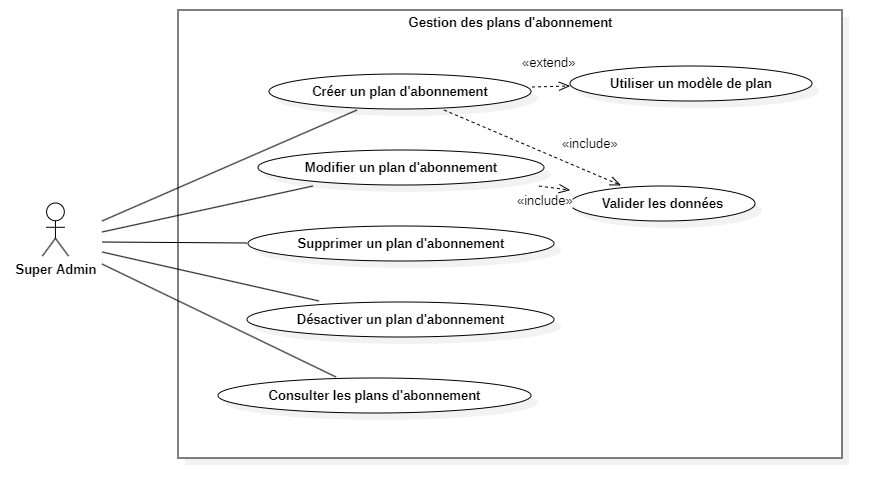
\includegraphics[width=12cm,height=8cm]{images/plansubscriptionuc.png}
    \caption{Diagramme de cas d'utilisation - Gestion des plans d'abonnement}
\end{figure}

\begin{longtable}{|>{\raggedright\arraybackslash}p{4cm}|>{\raggedright\arraybackslash}p{9cm}|}
\caption{Description textuelle du cas d'utilisation - Gestion des plans d'abonnement}
\label{tab:manage_subscription_plans_usecase} \\
\hline
\textbf{Cas d'utilisation} & \textbf{Gérer les plans d'abonnement} \\
\hline
\textbf{Acteur} & Super Admin \\
\hline
\textbf{Précondition} & Être authentifié en tant que Super Admin \\
\hline
\textbf{Postcondition} & Plans d'abonnement créés, modifiés, supprimés ou désactivés selon l'action \\
\hline
\textbf{Scénario nominal} & 
1. Le Super Admin accède à la page de gestion des plans d'abonnement \\
& 2. Le système affiche la liste des plans existants \\
& 3. Le Super Admin sélectionne une action (créer, modifier, supprimer, désactiver) \\
& 4. Le système affiche le formulaire correspondant \\
& 5. Le Super Admin saisit ou modifie les informations du plan \\
& 6. Le système valide les données (prix, limite d'utilisateurs, fonctionnalités) \\
& 7. Le système met à jour la base de données \\
& 8. Le système affiche un message de confirmation \\
\hline
\textbf{Scénario alternatif} & 
- Création : vérification de l'unicité du nom de plan \\
& - Modification : mise à jour des champs modifiables \\
& - Suppression : vérification qu'aucune entreprise n'utilise le plan \\
& - Désactivation : masquage du plan pour les nouvelles souscriptions \\
& - Utilisation de templates prédéfinis pour accélérer la création \\
\hline
\end{longtable}

\subsubsection{Diagramme de cas d'utilisation détaillé de la souscription aux abonnements}
\noindent La figure 4.2 présente le diagramme de cas d'utilisation détaillé pour la souscription aux abonnements par l'Admin.

\begin{figure}[H]
    \centering
    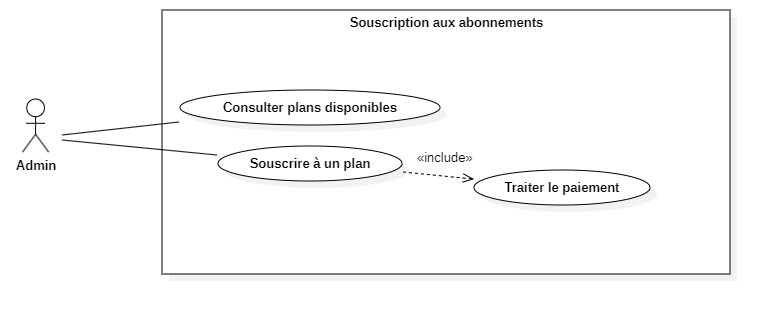
\includegraphics[width=11cm,height=7cm]{images/subscribeuc.png}
    \caption{Diagramme de cas d'utilisation - Souscription aux abonnements}
\end{figure}
\vspace{\baselineskip} 
\vspace{\baselineskip} 
\begin{longtable}{|>{\raggedright\arraybackslash}p{4cm}|>{\raggedright\arraybackslash}p{9cm}|}
\caption{Description textuelle du cas d'utilisation - Souscription aux abonnements}
\label{tab:subscribe_to_plans_usecase} \\
\hline
\textbf{Cas d'utilisation} & \textbf{Souscrire aux abonnements} \\
\hline
\textbf{Acteur} & Admin \\
\hline
\textbf{Précondition} & Être authentifié en tant qu'Admin \\
\hline
\textbf{Postcondition} & Abonnement souscrit et activé pour l'entreprise \\
\hline
\textbf{Scénario nominal} & 
1. L'Admin accède à la page des abonnements \\
& 2. Le système affiche les plans disponibles et l'abonnement actuel \\
& 3. L'Admin sélectionne un plan d'abonnement \\
& 4. Le système calcule le prix final (remise, taxes) \\
& 5. L'Admin confirme la souscription \\
& 6. Le système redirige vers Stripe pour le paiement \\
& 7. L'utilisateur effectue le paiement \\
& 8. Stripe confirme le paiement via webhook \\
& 9. Le système active l'abonnement \\
& 10. Le système affiche la confirmation d'activation \\
\hline
\textbf{Scénario alternatif} & 
- Paiement annulé : retour à la page des abonnements \\
& - Échec du paiement : affichage d'un message d'erreur \\
& - Vérification manuelle : endpoint de vérification de session \\
& - Abonnement existant : annulation de l'ancien abonnement \\
& - Gestion des erreurs de communication avec Stripe \\
\hline
\end{longtable}

\subsubsection{Diagramme de cas d'utilisation détaillé de la gestion des textes réglementaires}
\noindent La figure 4.3 présente le diagramme de cas d'utilisation détaillé pour la gestion des textes réglementaires par l'Admin et le Super Admin.

\begin{figure}[H]
    \centering
    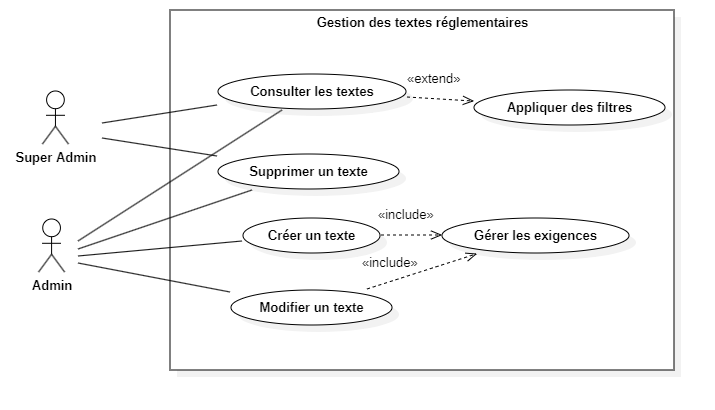
\includegraphics[width=12cm,height=8cm]{images/textsuc.png}
    \caption{Diagramme de cas d'utilisation - Gestion des textes réglementaires}
\end{figure}

\begin{longtable}{|>{\raggedright\arraybackslash}p{4cm}|>{\raggedright\arraybackslash}p{9cm}|}
\caption{Description textuelle du cas d'utilisation - Gestion des textes réglementaires}
\label{tab:manage_texts_usecase} \\
\hline
\textbf{Cas d'utilisation} & \textbf{Gérer les textes réglementaires} \\
\hline
\textbf{Acteur} & Admin, Super Admin \\
\hline
\textbf{Précondition} & Être authentifié en tant qu'Admin ou Super Admin \\
\hline
\textbf{Postcondition} & Textes réglementaires créés, modifiés, supprimés ou consultés selon l'action \\
\hline
\textbf{Scénario nominal} & 
1. L'utilisateur accède à la page de gestion des textes réglementaires \\
& 2. Le système affiche la liste des textes avec filtres \\
& 3. L'utilisateur sélectionne une action (créer, consulter, modifier, supprimer) \\
& 4. Le système affiche le formulaire ou les détails correspondants \\
& 5. L'utilisateur saisit ou modifie les informations du texte \\
& 6. Le système valide les données (domaine, thème, référence) \\
& 7. Le système met à jour la base de données \\
& 8. Le système affiche un message de confirmation \\
\hline
\textbf{Scénario alternatif} & 
- Création : ajout d'exigences et de pièces jointes \\
& - Consultation : marquage du texte comme consulté \\
& - Modification : mise à jour des champs éditables \\
& - Suppression : vérification des dépendances et suppression en cascade \\
& - Filtrage : par domaine, thème, statut, année de publication \\
& - Pagination : gestion des listes volumineuses \\
\hline
\end{longtable}

\subsubsection{Diagramme de cas d'utilisation détaillé de l'évaluation de conformité}
\noindent La figure 4.4 présente le diagramme de cas d'utilisation détaillé pour l'évaluation de conformité des textes réglementaires par l'Admin.

\begin{figure}[H]
    \centering
    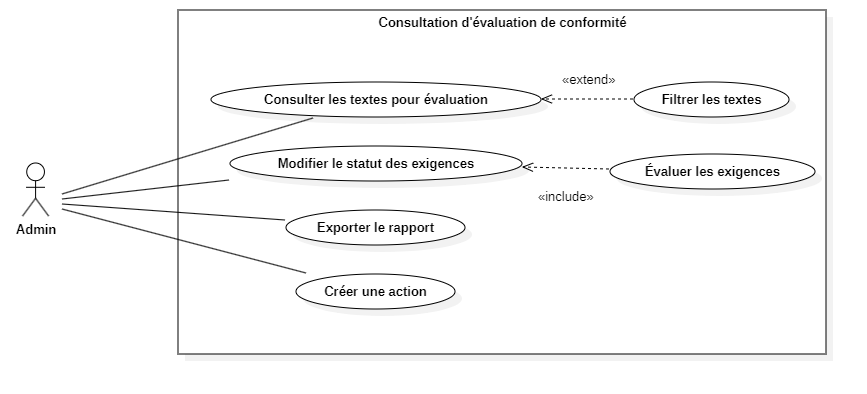
\includegraphics[width=12cm,height=8cm]{images/complianceuc.png}
    \caption{Diagramme de cas d'utilisation - Évaluation de conformité}
\end{figure}
\vspace{\baselineskip} 
\begin{longtable}{|>{\raggedright\arraybackslash}p{4cm}|>{\raggedright\arraybackslash}p{9cm}|}
\caption{Description textuelle du cas d'utilisation - Évaluation de conformité}
\label{tab:compliance_evaluation_usecase} \\
\hline
\textbf{Cas d'utilisation} & \textbf{Évaluer la conformité des textes} \\
\hline
\textbf{Acteur} & Admin \\
\hline
\textbf{Précondition} & Être authentifié en tant qu'Admin et avoir des textes réglementaires avec exigences \\
\hline
\textbf{Postcondition} & Statut de conformité mis à jour pour les exigences des textes réglementaires \\
\hline
\textbf{Scénario nominal} & 
1. L'Admin accède à la page d'évaluation de conformité \\
& 2. Le système affiche la liste des textes avec filtres et statuts \\
& 3. L'Admin sélectionne un texte à évaluer \\
& 4. Le système affiche les exigences du texte avec leur statut actuel \\
& 5. L'Admin modifie le statut d'une exigence (applicable, non-applicable, à vérifier, pour information) \\
& 6. Le système met à jour le statut dans la base de données \\
& 7. Le système recalcule le pourcentage d'applicabilité \\
& 8. Le système affiche la confirmation de mise à jour \\
\hline
\textbf{Scénario alternatif} & 
- Filtrage : par domaine, thème, nature, année de publication \\
& - Recherche : par mot-clé dans la référence ou le contenu \\
& - Pagination : navigation dans la liste des textes \\
& - Création d'actions : redirection vers le plan d'action \\
\hline
\end{longtable}

\subsubsection{Diagramme de cas d'utilisation détaillé de la gestion des plans d'action}
\noindent La figure 4.5 présente le diagramme de cas d'utilisation détaillé pour la gestion des plans d'action par l'Admin et l'Auditeur.

\begin{figure}[H]
    \centering
    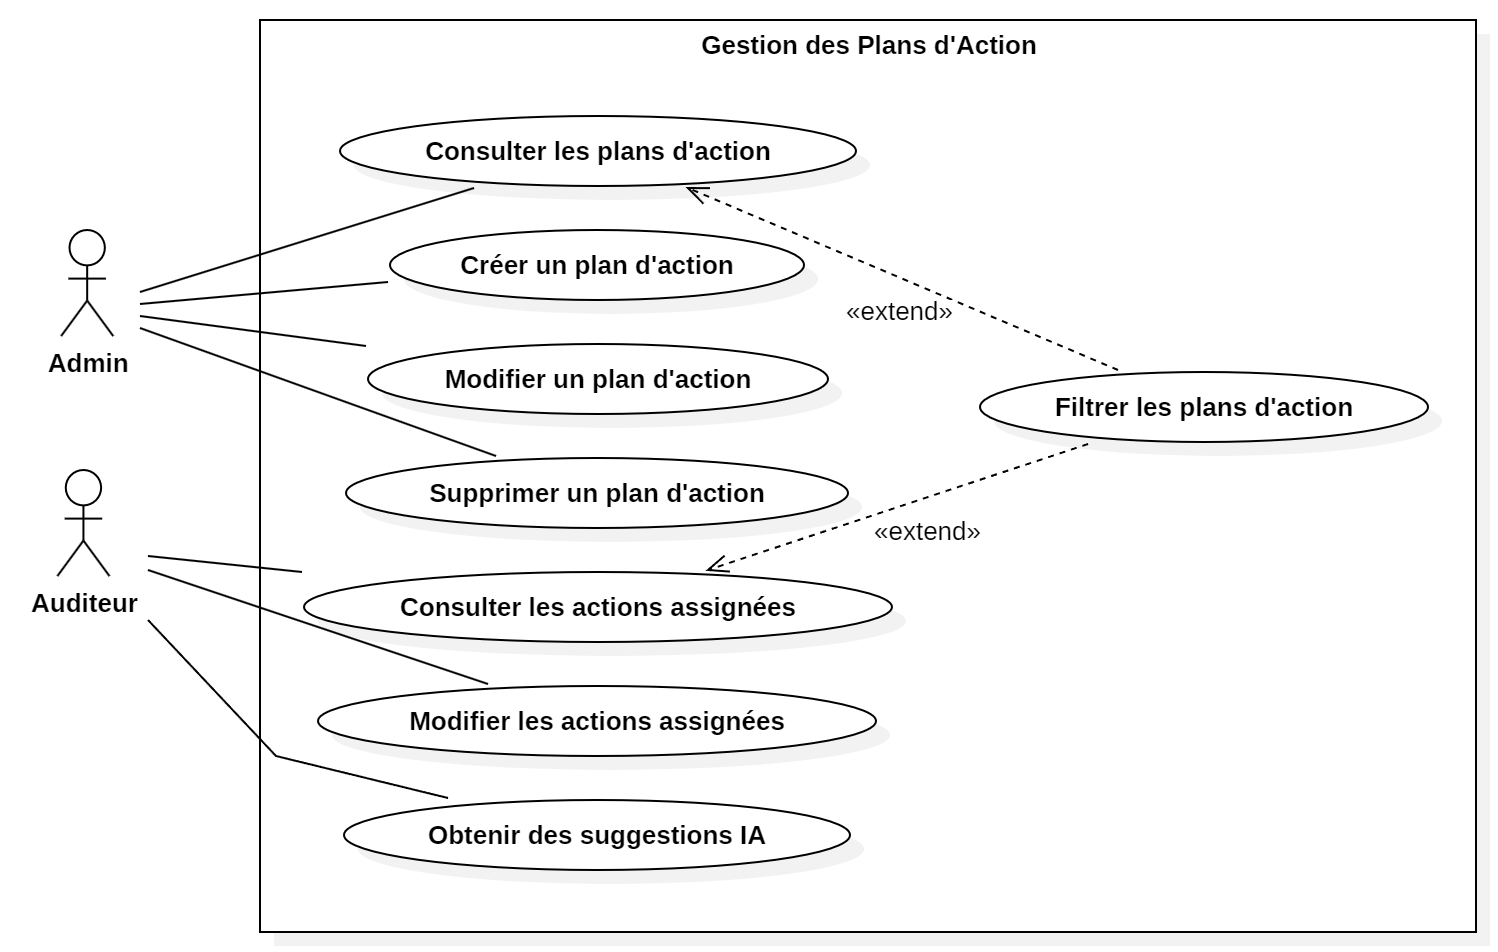
\includegraphics[width=14cm,height=10cm]{images/actionplansuc.png}
    \caption{Diagramme de cas d'utilisation - Gestion des plans d'action}
\end{figure}

\begin{longtable}{|>{\raggedright\arraybackslash}p{4cm}|>{\raggedright\arraybackslash}p{9cm}|}
\caption{Description textuelle du cas d'utilisation - Gestion des plans d'action}
\label{tab:manage_action_plans_usecase} \\
\hline
\textbf{Cas d'utilisation} & \textbf{Gérer les plans d'action} \\
\hline
\textbf{Acteur} & Admin, Auditeur \\
\hline
\textbf{Précondition} & Être authentifié en tant qu'Admin ou Auditeur \\
\hline
\textbf{Postcondition} & Plans d'action créés, modifiés, supprimés ou consultés selon l'action et le rôle \\
\hline
\textbf{Scénario nominal} & 
1. L'utilisateur accède à la page de gestion des plans d'action \\
& 2. Le système affiche la liste des actions selon les permissions \\
& 3. L'utilisateur sélectionne une action (créer, consulter, modifier, supprimer) \\
& 4. Le système affiche le formulaire ou les détails correspondants \\
& 5. L'utilisateur saisit ou modifie les informations de l'action \\
& 6. Le système valide les données (description, responsable, échéance) \\
& 7. Le système met à jour la base de données \\
& 8. Le système affiche un message de confirmation \\
\hline
\textbf{Scénario alternatif} & 
- Admin : gestion complète des actions de l'entreprise \\
& - Auditeur : consultation et modification des actions assignées uniquement \\
& - Filtrage : par statut, responsable, échéance, texte réglementaire \\
& - Conseils IA : génération automatique de recommandations pour les auditeurs \\
& - Pagination : gestion des listes volumineuses \\
& - Notifications : envoi automatique lors des assignations \\
\hline
\end{longtable}


\subsection{Conception}
\noindent Dans cette partie, nous passons à la seconde phase de notre sprint. Notre objectif est de créer les diagrammes de séquence correspondant à cette étape.

\subsubsection{Diagramme de séquence}

\subsubsection{Diagramme de séquence pour le scénario de création d'un plan d'abonnement}
\begin{figure}[H]
    \centering
    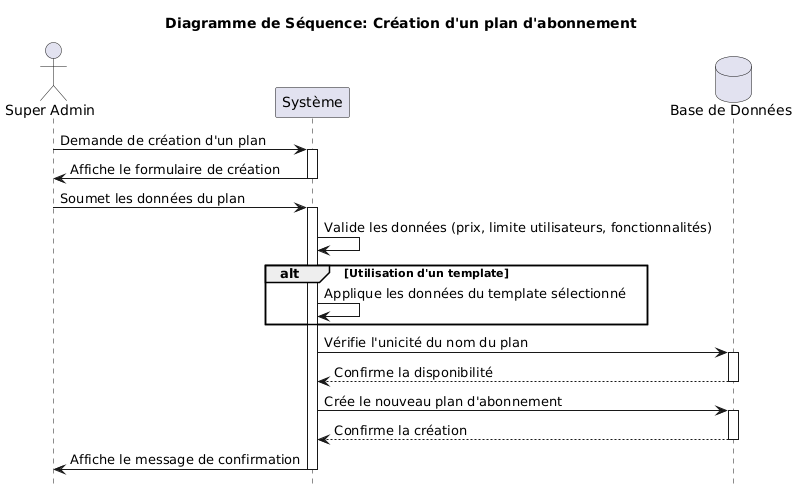
\includegraphics[width=10cm,height=9cm]{images/createplanseq.png}
    \caption{Diagramme de séquence pour le scénario de création d'un plan d'abonnement}
\end{figure}

\subsubsection{Diagramme de séquence pour le scénario de consultation des plans d'abonnement}
\begin{figure}[H]
    \centering
    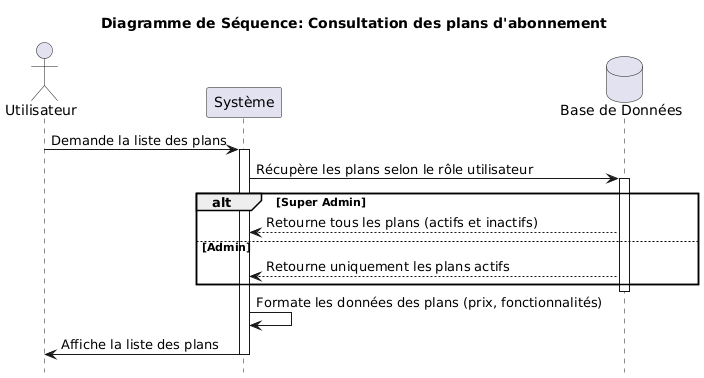
\includegraphics[width=9cm,height=8cm]{images/consultplanseq.png}
    \caption{Diagramme de séquence pour le scénario de consultation des plans d'abonnement}
\end{figure}

\subsubsection{Diagramme de séquence pour le scénario de modification d'un plan d'abonnement}
\begin{figure}[H]
    \centering
    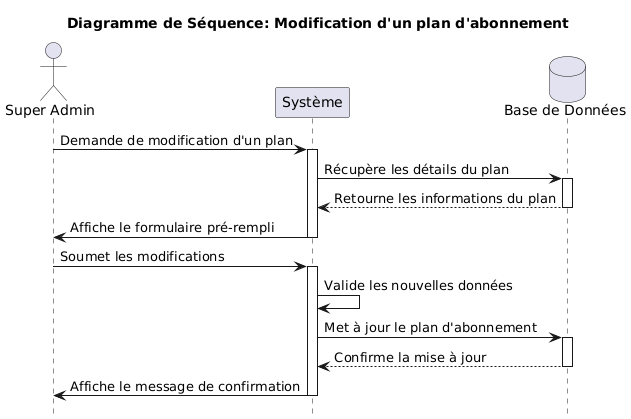
\includegraphics[width=10cm,height=9cm]{images/modifyplanseq.png}
    \caption{Diagramme de séquence pour le scénario de modification d'un plan d'abonnement}
\end{figure}

\subsubsection{Diagramme de séquence pour le scénario de suppression d'un plan d'abonnement}
\begin{figure}[H]
    \centering
    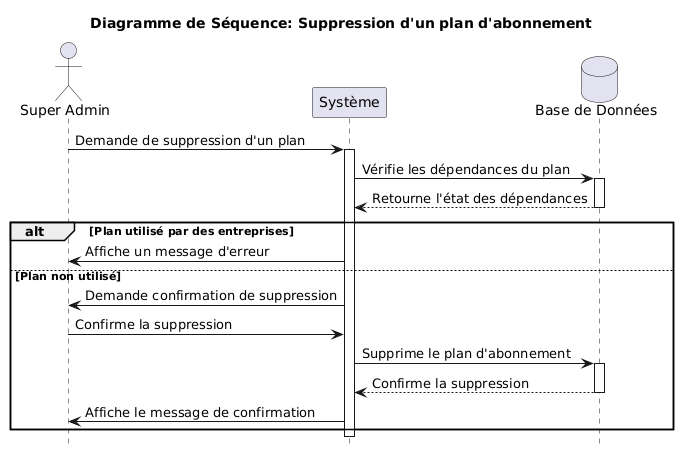
\includegraphics[width=10cm,height=9cm]{images/deleteplanseq.png}
    \caption{Diagramme de séquence pour le scénario de suppression d'un plan d'abonnement}
\end{figure}

\subsubsection{Diagramme de séquence pour le scénario de souscription à un abonnement}
\begin{figure}[H]
    \centering
    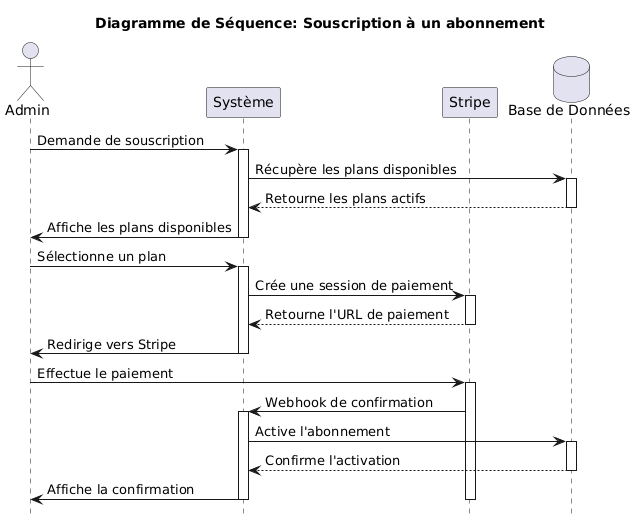
\includegraphics[width=10cm,height=9cm]{images/subscribeseq.png}
    \caption{Diagramme de séquence pour le scénario de souscription à un abonnement}
\end{figure}

\subsubsection{Diagramme de séquence pour le scénario de création d'un texte réglementaire}
\begin{figure}[H]
    \centering
    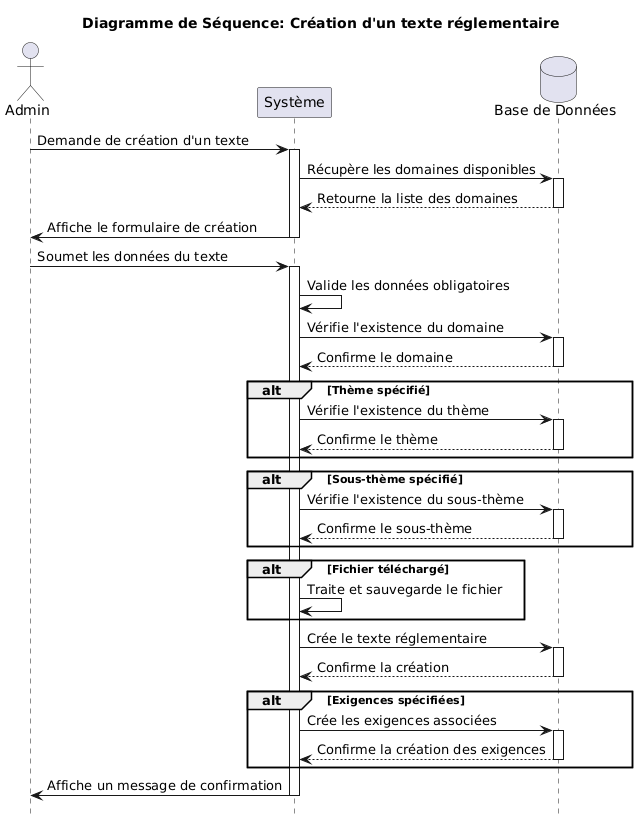
\includegraphics[width=10cm,height=9cm]{images/createtextseq.png}
    \caption{Diagramme de séquence pour le scénario de création d'un texte réglementaire}
\end{figure}

\subsubsection{Diagramme de séquence pour le scénario de consultation des textes réglementaires}
\begin{figure}[H]
    \centering
    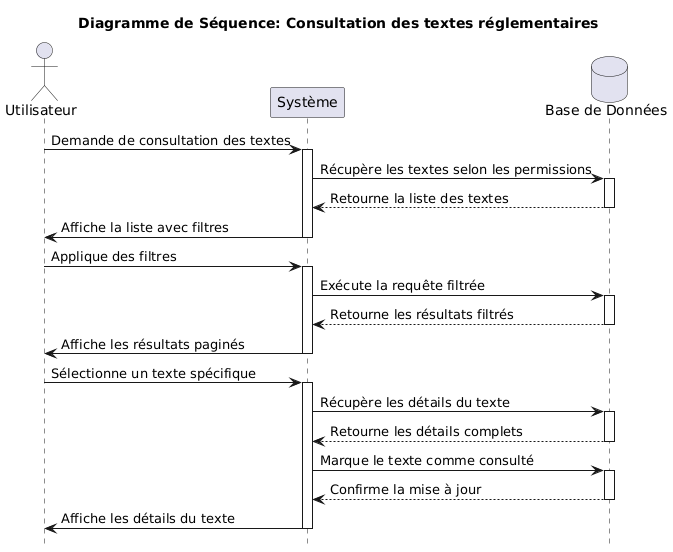
\includegraphics[width=10cm,height=9cm]{images/consulttextseq.png}
    \caption{Diagramme de séquence pour le scénario de consultation des textes réglementaires}
\end{figure}

\subsubsection{Diagramme de séquence pour le scénario de modification d'un texte réglementaire}
\begin{figure}[H]
    \centering
    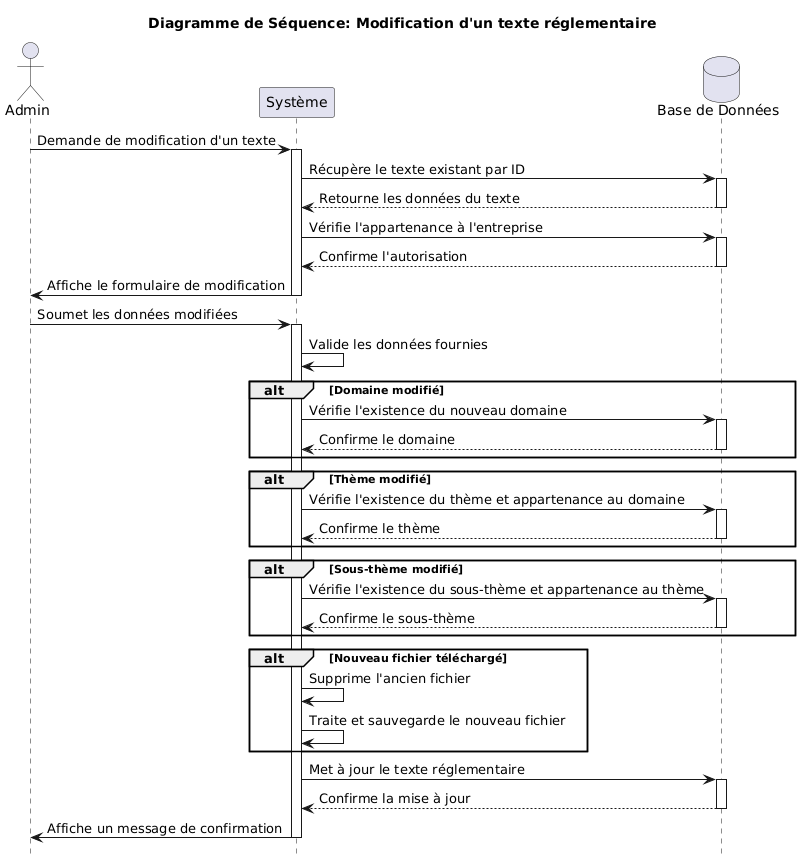
\includegraphics[width=10cm,height=9cm]{images/modifytextseq.png}
    \caption{Diagramme de séquence pour le scénario de modification d'un texte réglementaire}
\end{figure}

\subsubsection{Diagramme de séquence pour le scénario de suppression d'un texte réglementaire}
\begin{figure}[H]
    \centering
    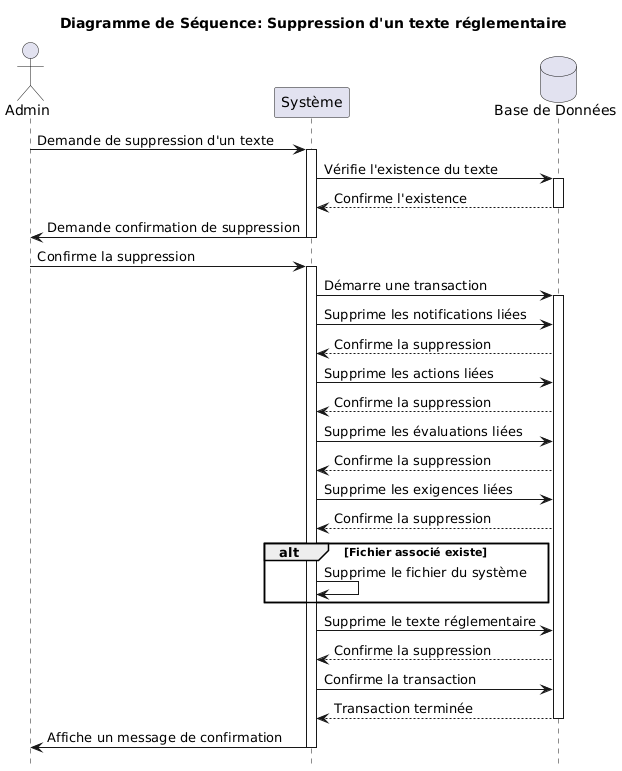
\includegraphics[width=10cm,height=9cm]{images/deletetextseq.png}
    \caption{Diagramme de séquence pour le scénario de suppression d'un texte réglementaire}
\end{figure}

\subsubsection{Diagramme de séquence pour le scénario d'évaluation de conformité}
\begin{figure}[H]
    \centering
    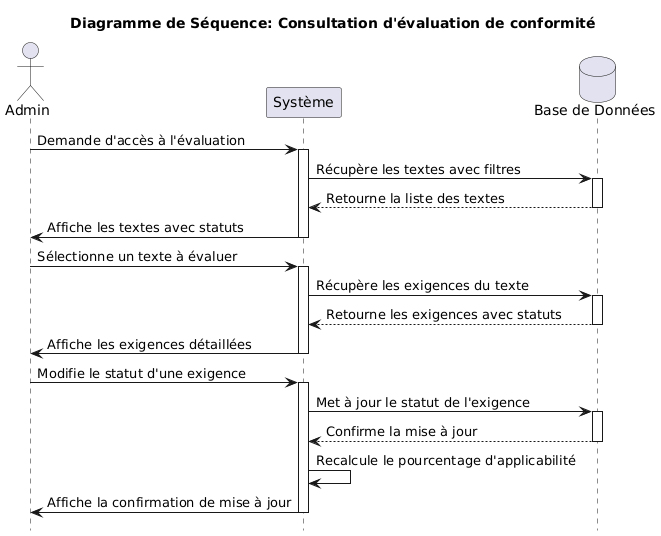
\includegraphics[width=10cm,height=9cm]{images/complianceseq.png}
    \caption{Diagramme de séquence pour le scénario d'évaluation de conformité}
\end{figure}

\subsubsection{Diagramme de séquence pour le scénario de création d'un plan d'action}
\begin{figure}[H]
    \centering
    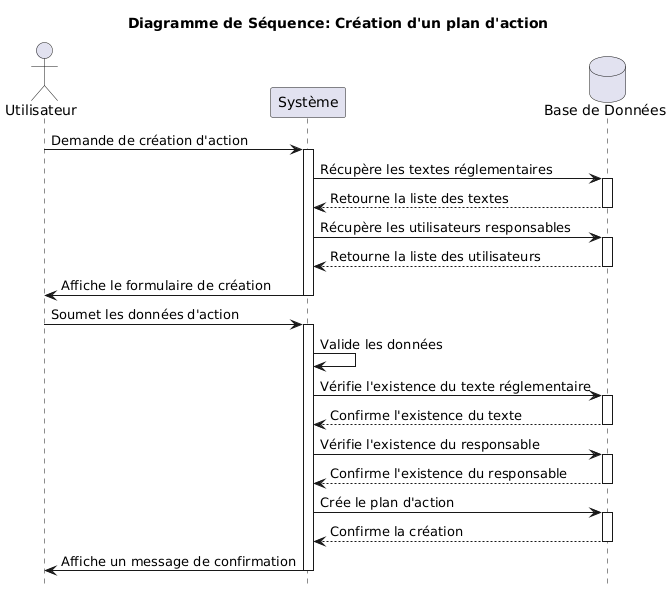
\includegraphics[width=10cm,height=9cm]{images/createactionseq.png}
    \caption{Diagramme de séquence pour le scénario de création d'un plan d'action}
\end{figure}

\subsubsection{Diagramme de séquence pour le scénario de consultation des plans d'action}
\begin{figure}[H]
    \centering
    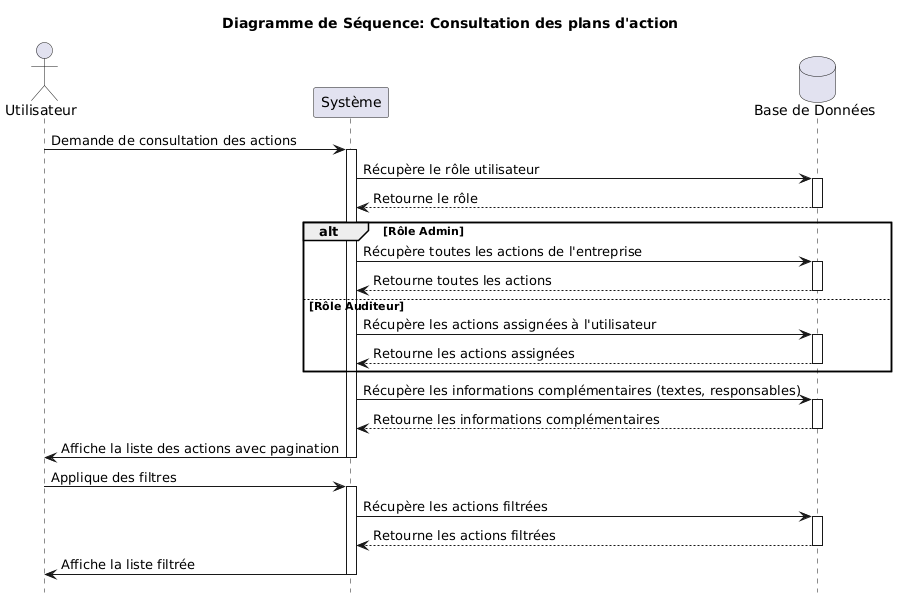
\includegraphics[width=10cm,height=9cm]{images/consultactionseq.png}
    \caption{Diagramme de séquence pour le scénario de consultation des plans d'action}
\end{figure}

\subsubsection{Diagramme de séquence pour le scénario de modification d'un plan d'action}
\begin{figure}[H]
    \centering
    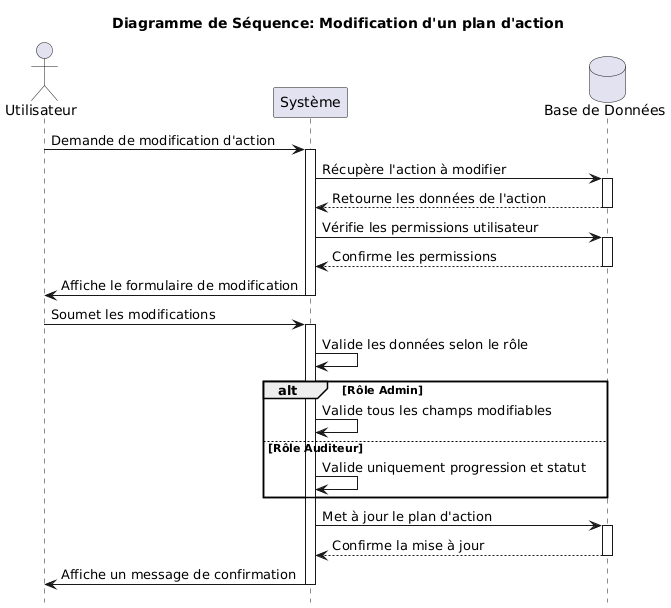
\includegraphics[width=10cm,height=9cm]{images/modifyactionseq.png}
    \caption{Diagramme de séquence pour le scénario de modification d'un plan d'action}
\end{figure}

\subsubsection{Diagramme de séquence pour le scénario de suppression d'un plan d'action}
\begin{figure}[H]
    \centering
    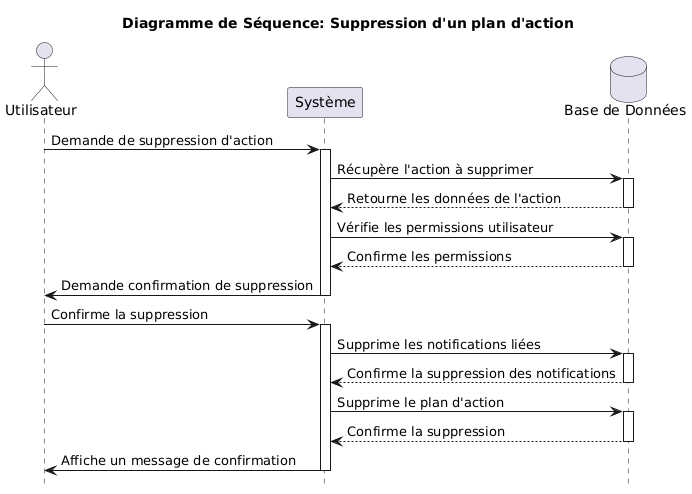
\includegraphics[width=10cm,height=9cm]{images/deleteactionseq.png}
    \caption{Diagramme de séquence pour le scénario de suppression d'un plan d'action}
\end{figure}
\subsubsection{Diagramme de séquence pour le scénario de génération de conseils IA}
\begin{figure}[H]
    \centering
    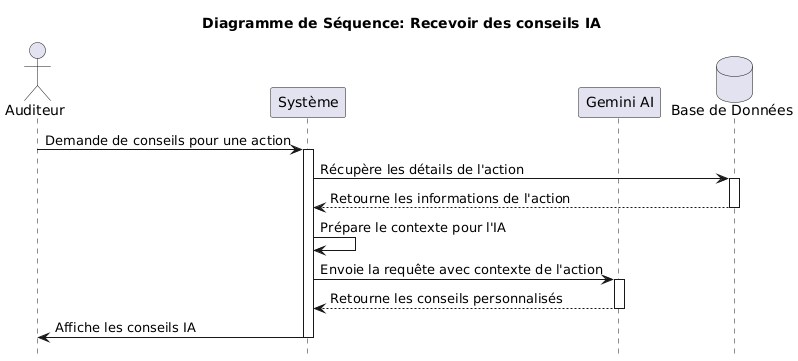
\includegraphics[width=13cm,height=10cm]{images/aiconseilseq.png}
    \caption{Diagramme de séquence pour le scénario de génération de conseils IA}
\end{figure}

\subsection{Réalisation}
\noindent Dans cette section, nous allons vous présenter de manière progressive et détaillée les résultats obtenus au cours de ce sprint. Ces résultats seront exposés sous la forme d’une série de captures d’écran illustrant plus clairement les différentes interfaces que nous avons développées durant cette phase.

\subsubsection{Interface de gestion des plans d'abonnement}
\noindent La figure 4.6 met en évidence l’interface dédiée à la gestion des plans d’abonnement destinée au Super Administrateur. Cette interface lui permet de créer de nouveaux plans, de modifier ceux qui existent déjà, ainsi que de procéder à la suppression des plans devenus inutiles.

\begin{figure}[H]
    \centering
    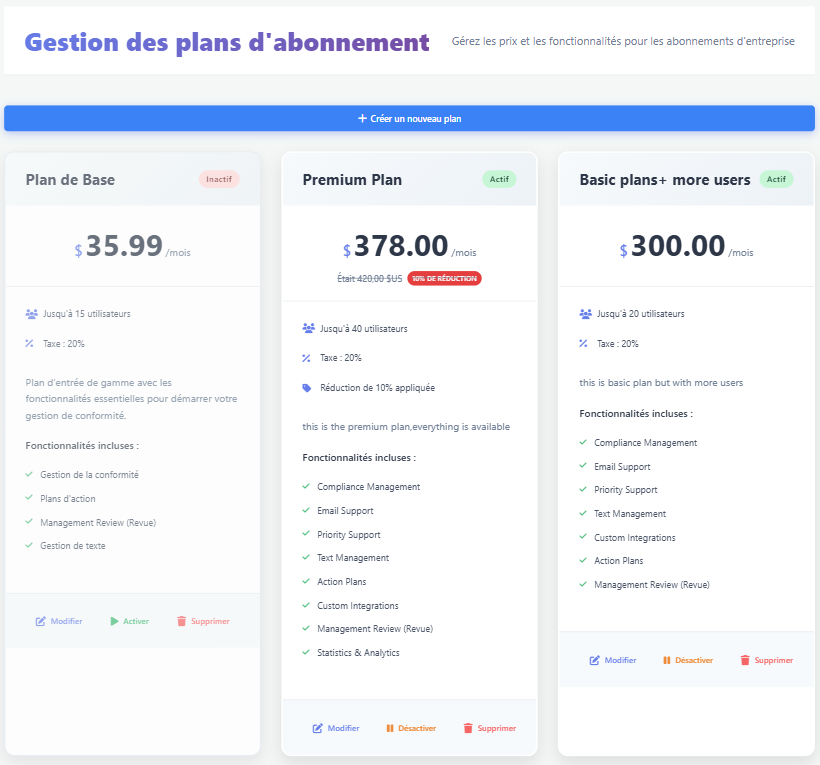
\includegraphics[width=13cm,height=9cm]{images/gestionplansinterface.PNG}
    \caption{Interface de gestion des plans d'abonnement}
\end{figure}

\subsubsection{Interface de création d'un plan d'abonnement}
\noindent La figure 4.7 présente l'interface de création d'un nouveau plan d'abonnement avec tous les champs nécessaires.

\begin{figure}[H]
    \centering
    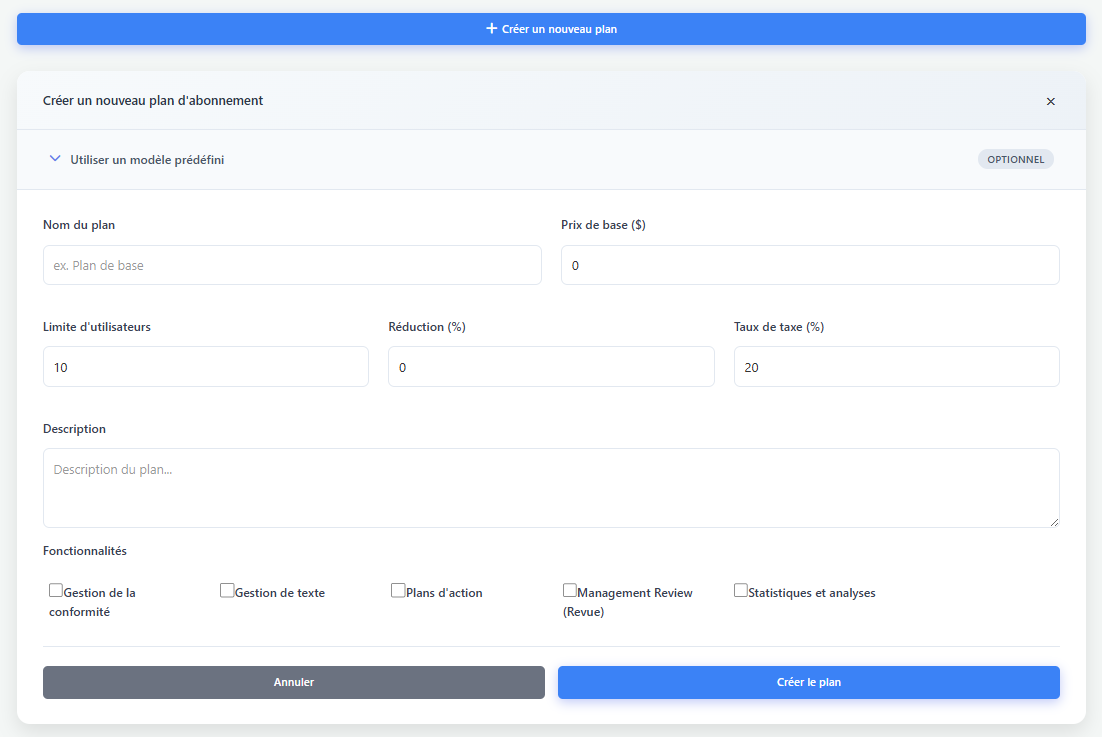
\includegraphics[width=13cm,height=9cm]{images/createplanmodal.PNG}
    \caption{Interface de création d'un plan d'abonnement}
\end{figure}

\subsubsection{Interface de souscription aux abonnements}
\noindent La figure 4.9 présente l'interface de souscription aux abonnements pour l'Admin permettant de visualiser et souscrire aux plans disponibles.

\begin{figure}[H]
    \centering
    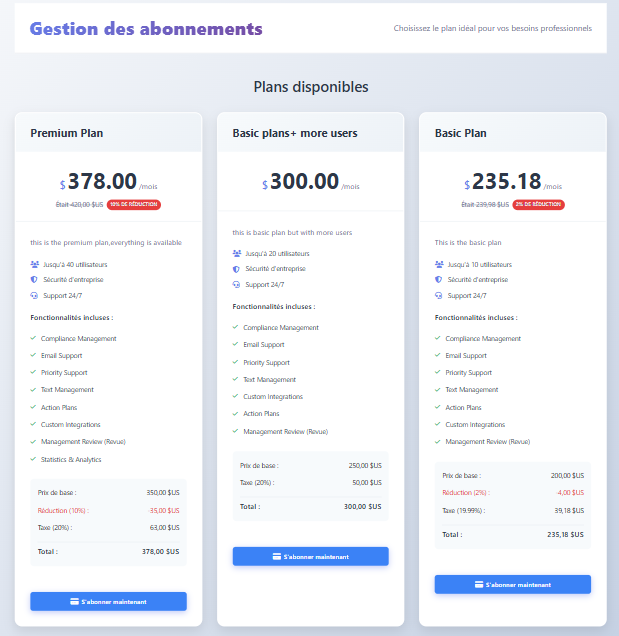
\includegraphics[width=11cm,height=8cm]{images/subscriptioninterface.PNG}
    \caption{Interface de souscription aux abonnements}
\end{figure}

\subsubsection{Interface de gestion des textes réglementaires}
\noindent La figure 4.10 présente l'interface de gestion des textes réglementaires permettant de consulter, filtrer et gérer les textes.

\begin{figure}[H]
    \centering
    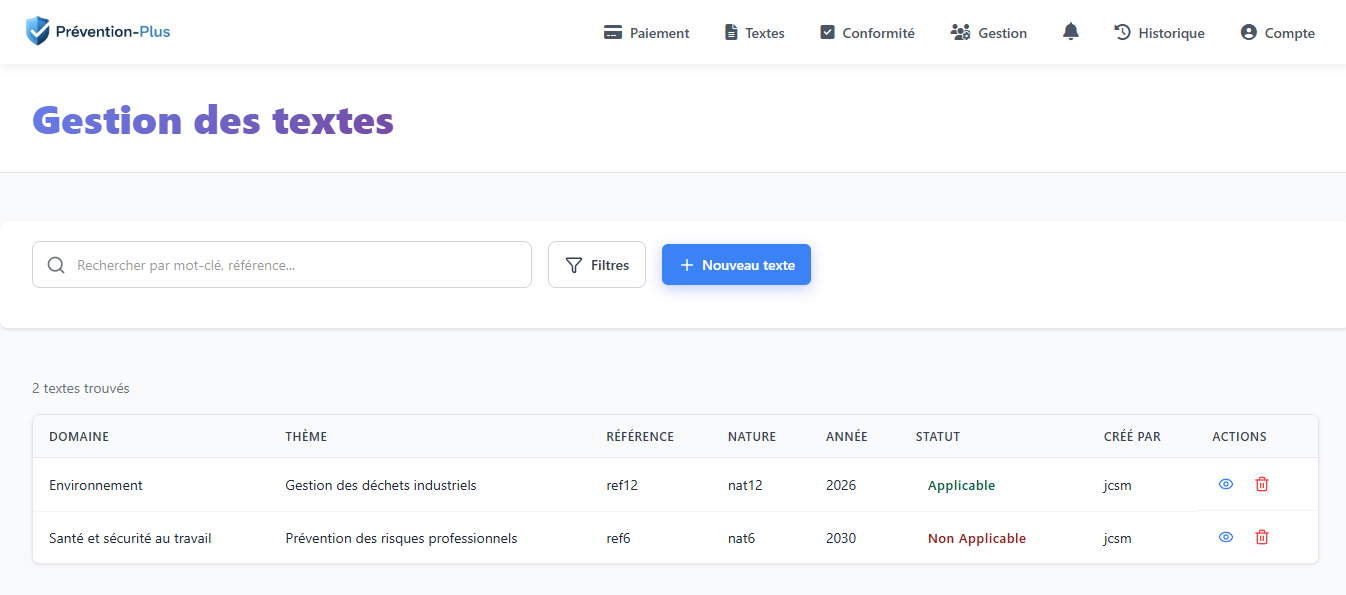
\includegraphics[width=12cm,height=7cm]{images/textsinterface.PNG}
    \caption{Interface de gestion des textes réglementaires}
\end{figure}

\subsubsection{Interface de création d'un texte réglementaire}
\noindent La figure 4.11 présente l'interface de création d'un nouveau texte réglementaire avec tous les champs nécessaires.

\begin{figure}[H]
    \centering
    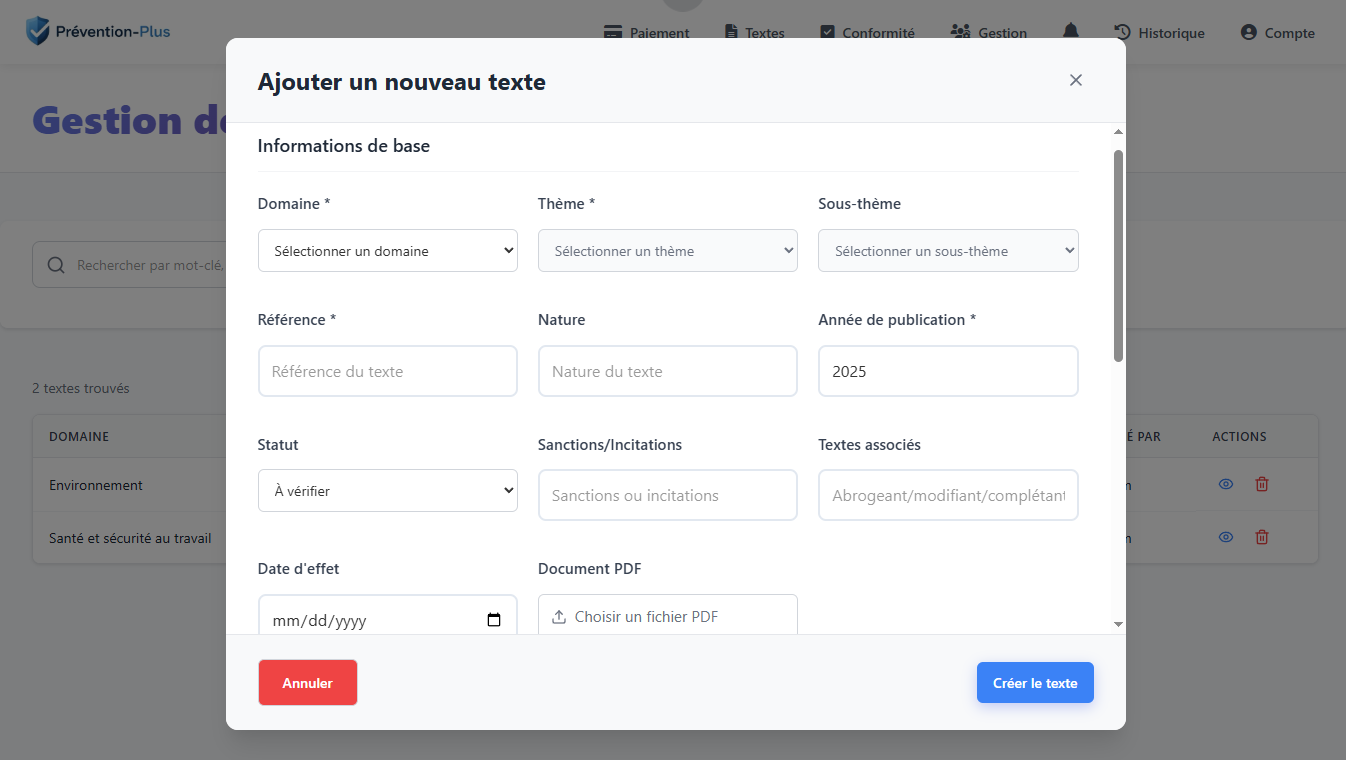
\includegraphics[width=12cm,height=7cm]{images/createtextmodal.PNG}
    \caption{Interface de création d'un texte réglementaire}
\end{figure}

\subsubsection{Interface d'évaluation de conformité}
\noindent La figure 4.14 présente l'interface d'évaluation de conformité permettant de consulter et évaluer les textes réglementaires.

\begin{figure}[H]
    \centering
    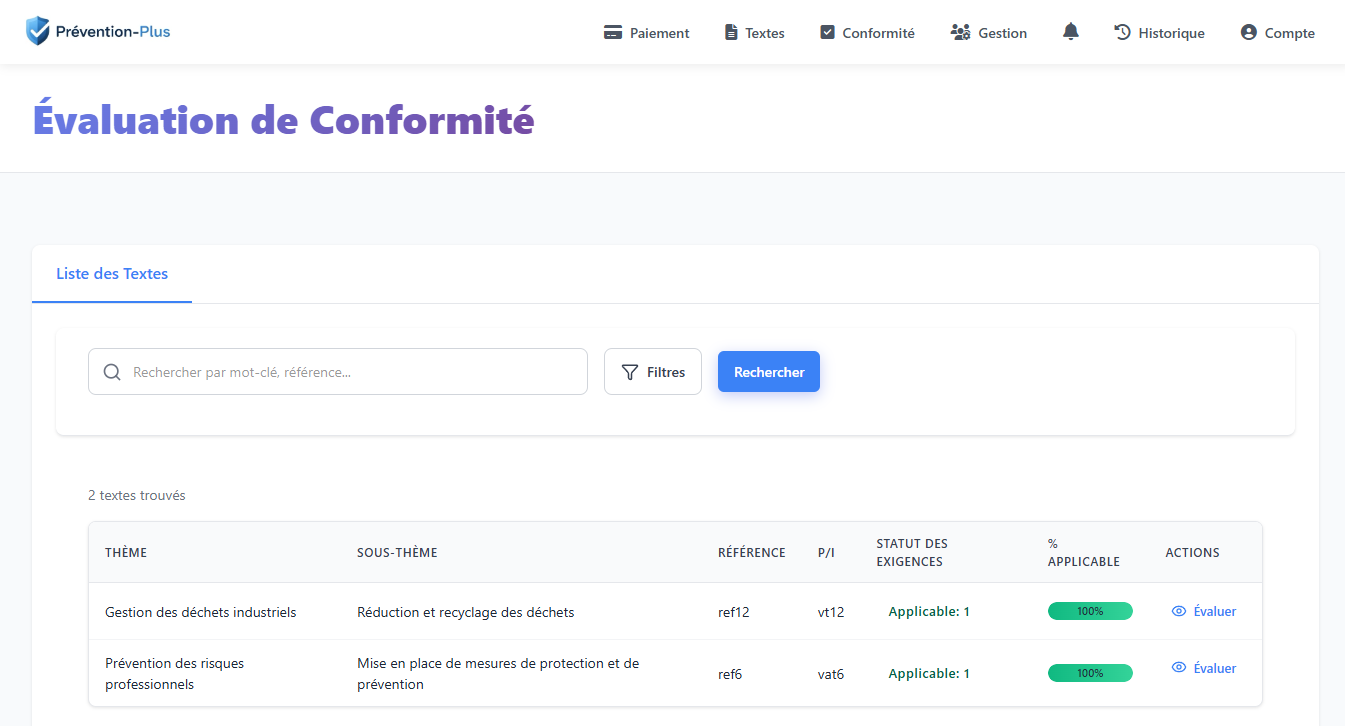
\includegraphics[width=13cm,height=8cm]{images/complianceinterface.PNG}
    \caption{Interface d'évaluation de conformité}
\end{figure}

\subsubsection{Interface d'évaluation des exigences}
\noindent La figure 4.15 présente l'interface d'évaluation des exigences d'un texte réglementaire spécifique.

\begin{figure}[H]
    \centering
    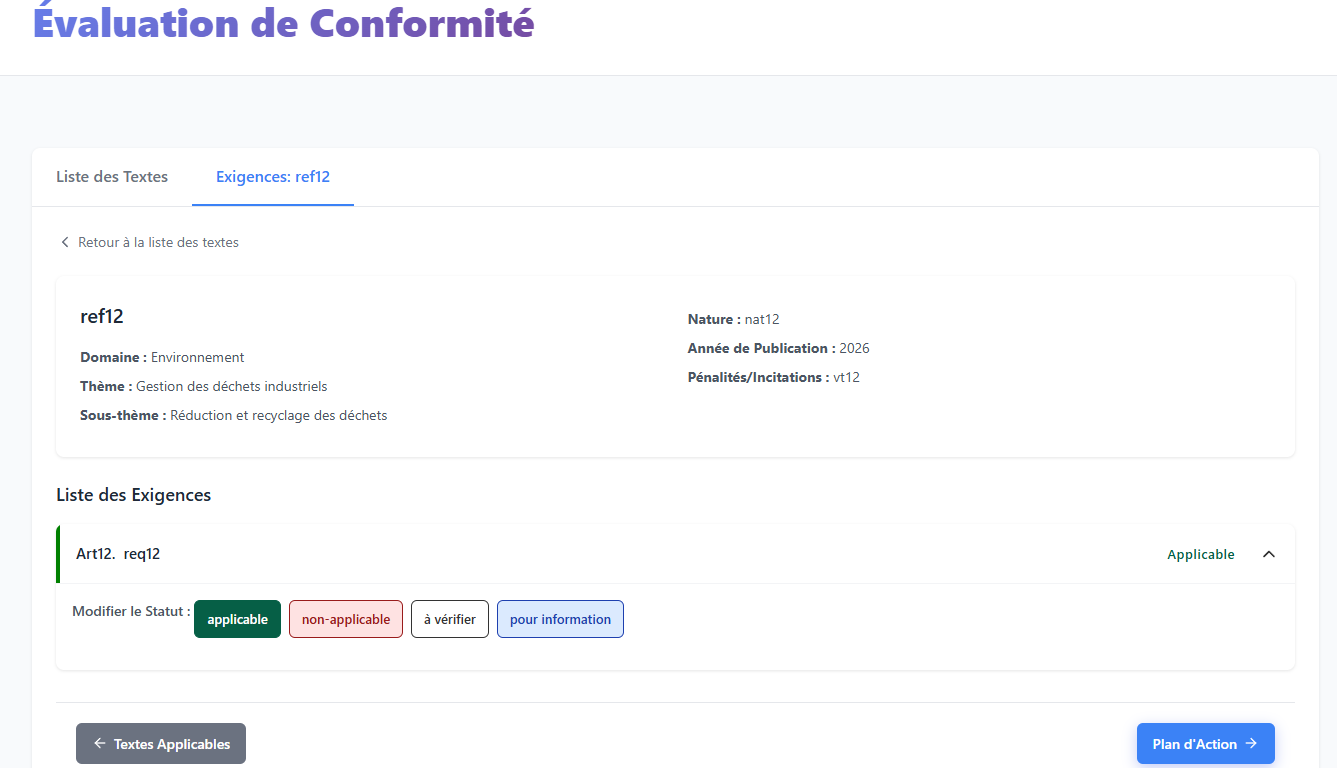
\includegraphics[width=13cm,height=8cm]{images/requirementevaluation.PNG}
    \caption{Interface d'évaluation des exigences}
\end{figure}

\subsubsection{Interface de gestion des plans d'action}
\noindent La figure 4.17 présente l'interface de gestion des plans d'action permettant de consulter, créer et gérer les actions.

\begin{figure}[H]
    \centering
    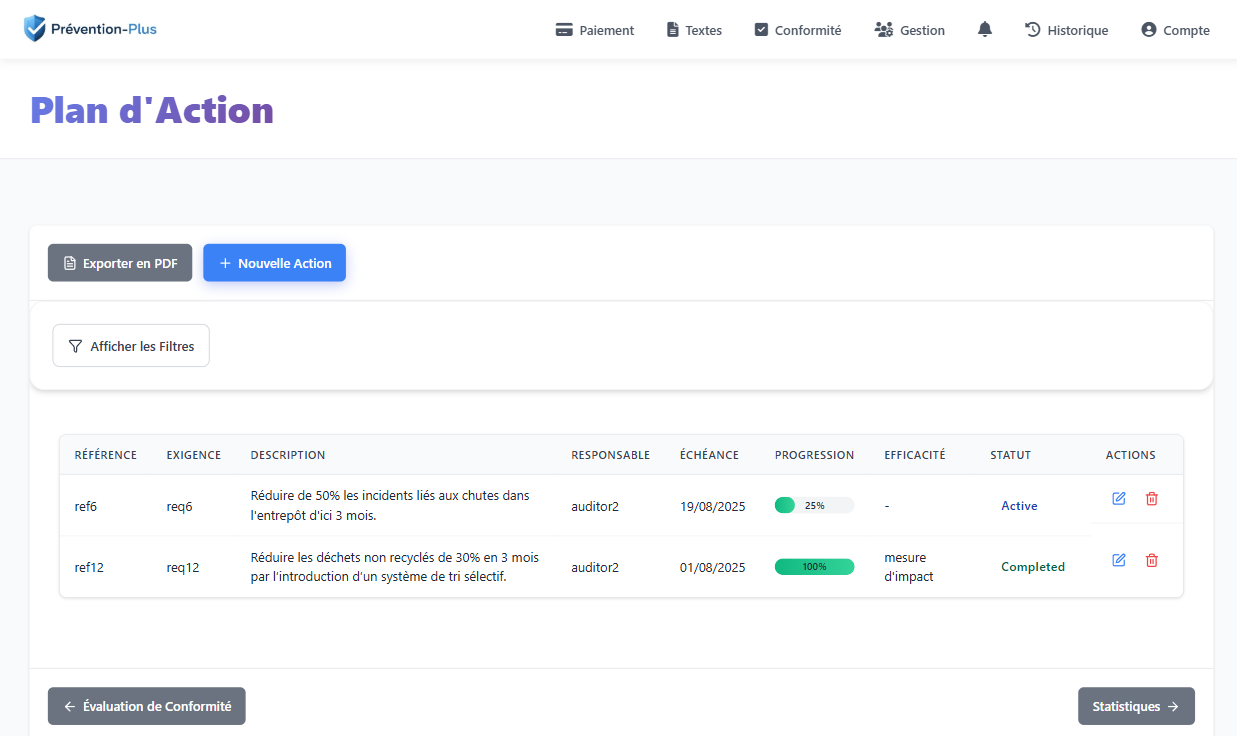
\includegraphics[width=13cm,height=8cm]{images/actionplansinterface.PNG}
    \caption{Interface de gestion des plans d'action}
\end{figure}

\subsubsection{Interface de création d'un plan d'action}
\noindent La figure 4.18 présente l'interface de création d'un nouveau plan d'action avec tous les champs nécessaires.

\begin{figure}[H]
    \centering
    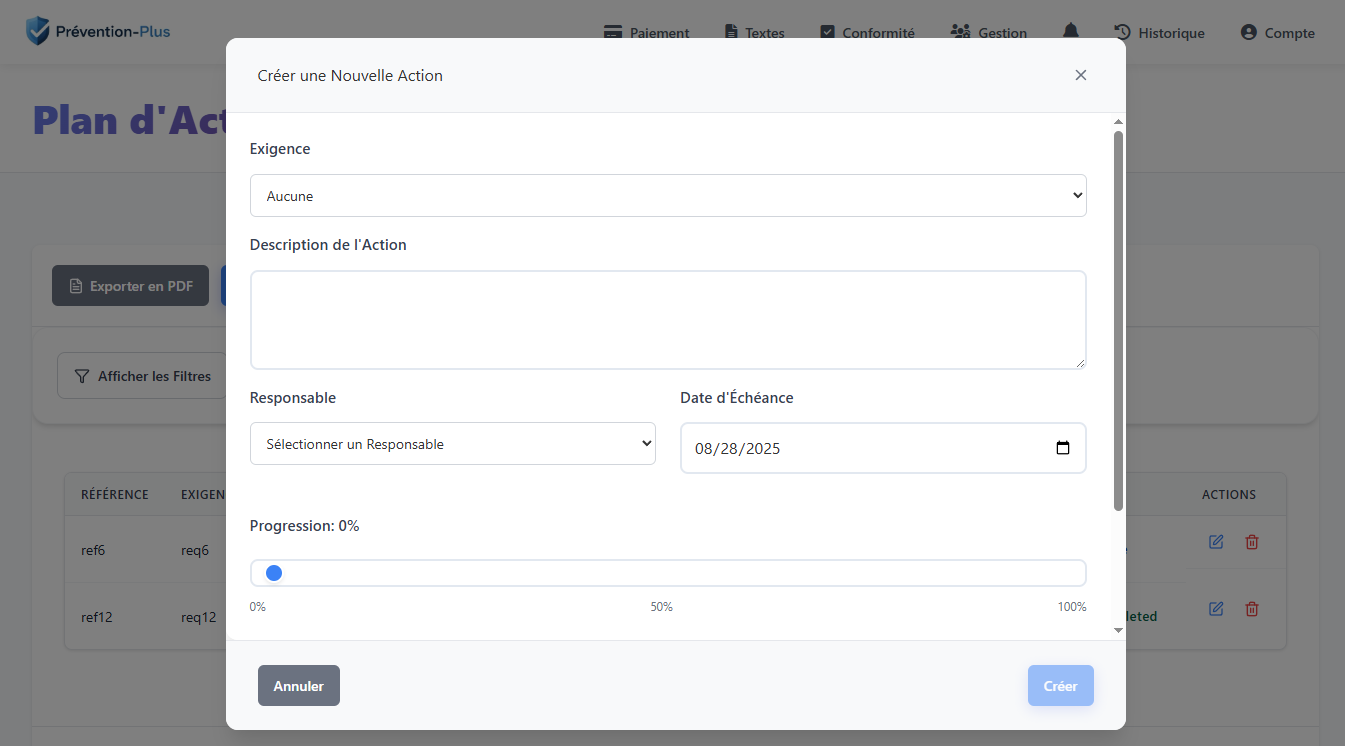
\includegraphics[width=13cm,height=7cm]{images/createactionmodal.PNG}
    \caption{Interface de création d'un plan d'action}
\end{figure}
\subsubsection{Interface des conseils IA pour les plans d'action}
La figure 4.16 présente l'interface des conseils IA permettant aux auditeurs de recevoir des recommandations personnalisées pour optimiser leurs actions.

\begin{figure}[H]
    \centering
    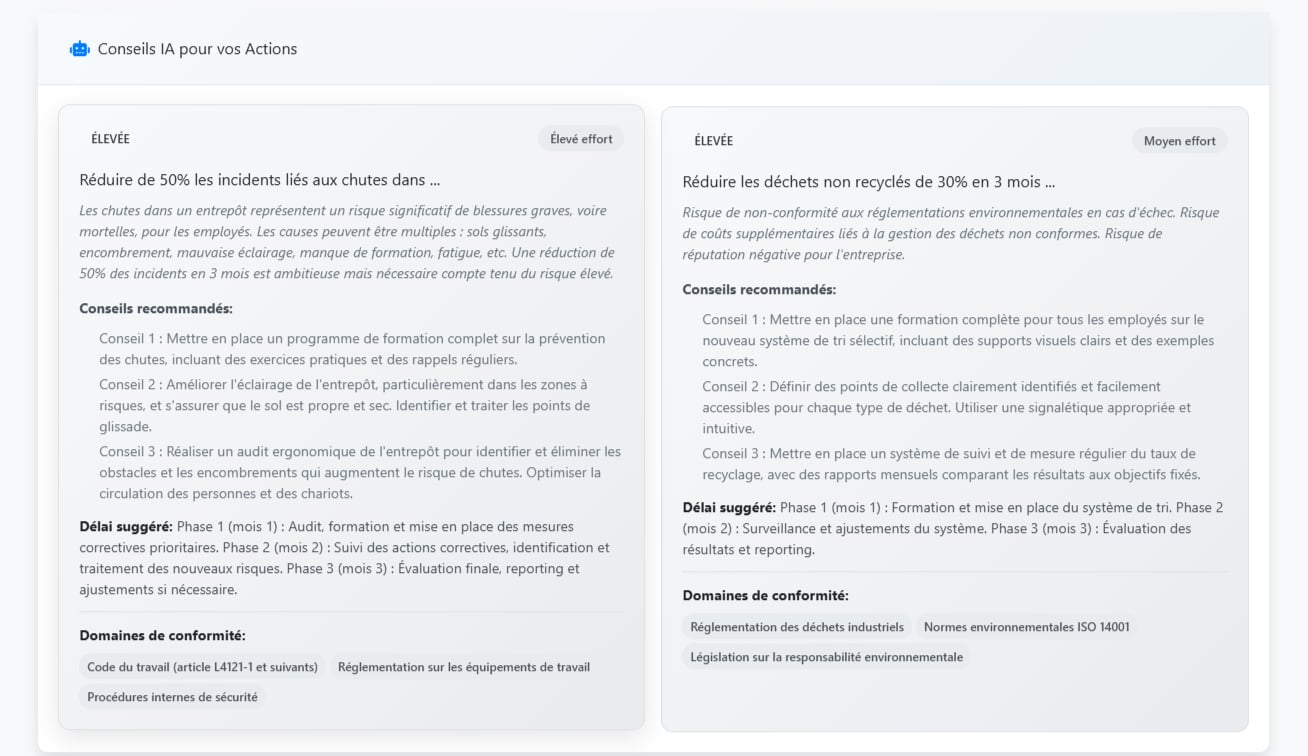
\includegraphics[width=13cm,height=8cm]{images/actionplanaiconseil.png
}
    \caption{Interface des conseils IA pour les plans d'action}
\end{figure}

\section{Sprint 2 : Gestion des revues de direction, notifications, historique et statistiques}

\subsection{Spécifications fonctionnelles}
\noindent Ce sprint représente la deuxième phase de notre deuxième release, établissant les mécanismes de gestion des revues de direction, des notifications, de consultation de l'historique et des statistiques, permettant aux entreprises d'organiser et de suivre les processus d'évaluation périodique tout en assurant une communication efficace, la traçabilité des actions et l'analyse des données de conformité.

\subsubsection{Backlog du Sprint 2}
\noindent Le sprint backlog est constitué à partir du backlog produit présenté au chapitre 2. Pour ce deuxième sprint de la release 2, nous avons sélectionné les user stories présentées dans le tableau 4.21.

\begin{longtable}{|>{\raggedright\arraybackslash}p{4cm}|>{\raggedright\arraybackslash}p{7cm}|>{\raggedright\arraybackslash}p{2cm}|}
\caption{Backlog du sprint 2 - Release 2}
\label{tab:sprint2_release2_backlog}\\
\hline
Histoire utilisateur & Description & Priorité \\
\hline
\endfirsthead
\multicolumn{3}{c}{\tablename\ \thetable\ -- suite} \\
\hline
Histoire utilisateur & Description & Priorité \\
\hline
\endhead
Gérer les revues de direction & En tant qu'Admin, je veux créer des revues de direction pour organiser les évaluations & Moyenne \\
\hline
Participer aux revues de direction & En tant qu'Admin, je veux participer aux revues et marquer leur statut comme complété ou annulé pour gérer le processus d'évaluation & Moyenne \\
\hline
Participer aux revues de direction & En tant qu'Auditeur, je veux participer aux revues en consultant, créant, modifiant et supprimant les éléments pour contribuer au processus d'évaluation & Moyenne \\
\hline
Gérer les notifications & En tant qu'utilisateur, je veux consulter mes notifications pour rester informé des activités du système & Faible \\
\hline
Consulter l'historique & En tant que Super Admin, je veux consulter l'historique complet des utilisateurs du site pour assurer la supervision & Moyenne \\
\hline
Consulter l'historique & En tant qu'Admin, je veux consulter l'historique des utilisateurs de mon entreprise pour assurer la traçabilité & Moyenne \\
\hline
Consulter l'historique & En tant qu'Auditeur, je veux consulter mon historique pour suivre mes actions & Moyenne \\
\hline
Consulter les statistiques & En tant que Super Admin, je veux consulter les statistiques globales du système pour analyser les performances & Faible \\
\hline
Consulter les statistiques & En tant qu'Admin, je veux consulter les statistiques de conformité de mon entreprise pour analyser les performances & Faible \\
\hline
\end{longtable}
\subsubsection{Diagramme de cas d'utilisation détaillé de la gestion des revues de direction}
\noindent La figure 4.21 présente le diagramme de cas d'utilisation détaillé pour la gestion des revues de direction par l'Admin.

\begin{figure}[H]
    \centering
    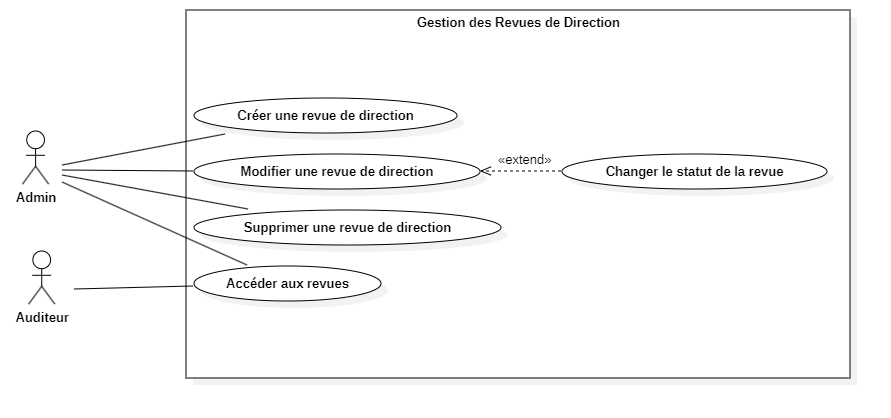
\includegraphics[width=11cm,height=7cm]{images/revuedirectionuc.png}
    \caption{Diagramme de cas d'utilisation - Gestion des revues de direction}
\end{figure}


\begin{longtable}{|>{\raggedright\arraybackslash}p{4cm}|>{\raggedright\arraybackslash}p{9cm}|}
\caption{Description textuelle du cas d'utilisation - Gestion des revues de direction}
\label{tab:manage_direction_reviews_usecase} \\
\hline
\textbf{Cas d'utilisation} & \textbf{Gérer les revues de direction} \\
\hline
\textbf{Acteur} & Admin \\
\hline
\textbf{Précondition} & Être authentifié en tant qu'Admin \\
\hline
\textbf{Postcondition} & Revues de direction créées, modifiées ou supprimées selon l'action \\
\hline
\textbf{Scénario nominal} & 
1. L'Admin accède à la page de gestion des revues de direction \\
& 2. L'Admin sélectionne une action (créer, modifier, supprimer) \\
& 3. Le système affiche le formulaire correspondant \\
& 4. L'Admin saisit ou modifie les informations de la revue \\
& 5. Le système valide les données (domaine, date de revue, statut) \\
& 6. Le système met à jour la base de données \\
& 7. Le système affiche un message de confirmation \\
\hline
\textbf{Scénario alternatif} & 
- Création : sélection du domaine et définition de la date \\
& - Modification : mise à jour des champs éditables (date, statut) \\
& - Suppression : vérification des permissions et suppression complète \\
& - Changement de statut : Draft → In Progress → Completed/Canceled \\
& - Validation des rôles : seuls les Admins peuvent modifier les statuts \\
\hline
\end{longtable}

\subsubsection{Diagramme de cas d'utilisation détaillé de la participation aux revues de direction}
\noindent La figure 4.22 présente le diagramme de cas d'utilisation détaillé pour la participation aux revues de direction par l'Admin et l'Auditeur.

\begin{figure}[H]
    \centering
    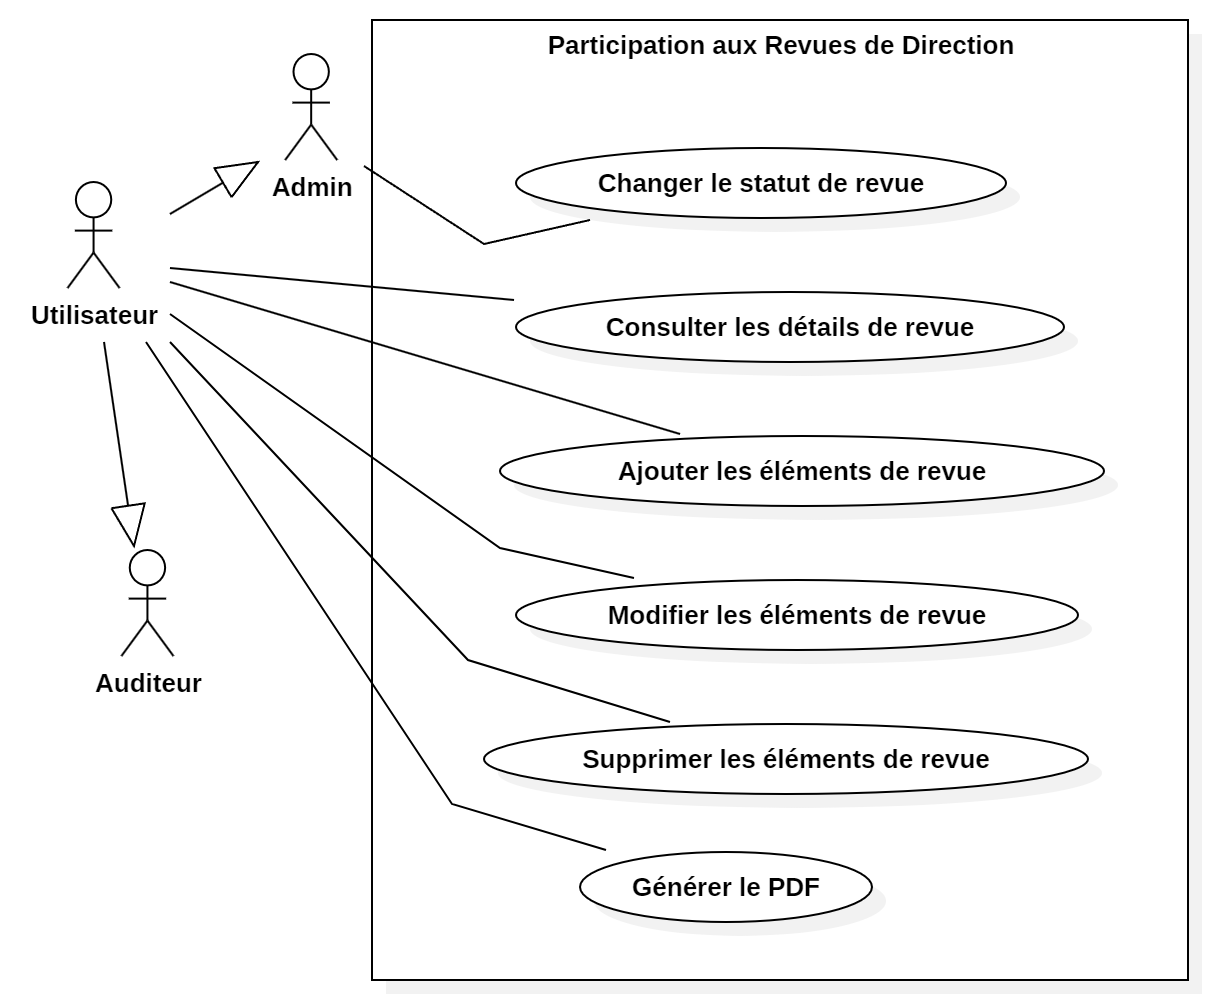
\includegraphics[width=11cm,height=7cm]{images/participationrevueuc.png}
    \caption{Diagramme de cas d'utilisation - Participation aux revues de direction}
\end{figure}

\begin{longtable}{|>{\raggedright\arraybackslash}p{4cm}|>{\raggedright\arraybackslash}p{9cm}|}
\caption{Description textuelle du cas d'utilisation - Participation aux revues de direction}
\label{tab:participate_direction_reviews_usecase} \\
\hline
\textbf{Cas d'utilisation} & \textbf{Participer aux revues de direction} \\
\hline
\textbf{Acteur} & Admin, Auditeur \\
\hline
\textbf{Précondition} & Être authentifié en tant qu'Admin ou Auditeur et la revue doit exister \\
\hline
\textbf{Postcondition} & Éléments de revue consultés, créés, modifiés ou supprimés selon l'action \\
\hline
\textbf{Scénario nominal} & 
1. L'utilisateur accède à la page de détails d'une revue de direction \\
& 2. Le système affiche les détails de la revue et ses éléments \\
& 3. L'utilisateur consulte les éléments ou sélectionne une action (ajouter, modifier, supprimer) \\
& 4. Le système affiche le formulaire ou les détails correspondants \\
& 5. L'utilisateur saisit ou modifie les informations si nécessaire \\
& 6. Le système valide les données et met à jour la base de données \\
& 7. Le système affiche un message de confirmation \\
\hline
\textbf{Scénario alternatif} & 
- Changement de statut : uniquement par Admin \\
& - Génération PDF : uniquement pour revues complétées ou annulées \\
& - Suppression d'éléments : vérification des permissions (créateur ou Admin) \\
& - Ajout d'éléments : uniquement si la revue est "En cours" \\
& - Modification d'éléments : uniquement si la revue est "En cours" \\
\hline
\end{longtable}

\subsubsection{Diagramme de cas d'utilisation détaillé de la gestion des notifications}
\noindent La figure 4.23 présente le diagramme de cas d'utilisation détaillé pour la gestion des notifications.

\begin{figure}[H]
    \centering
    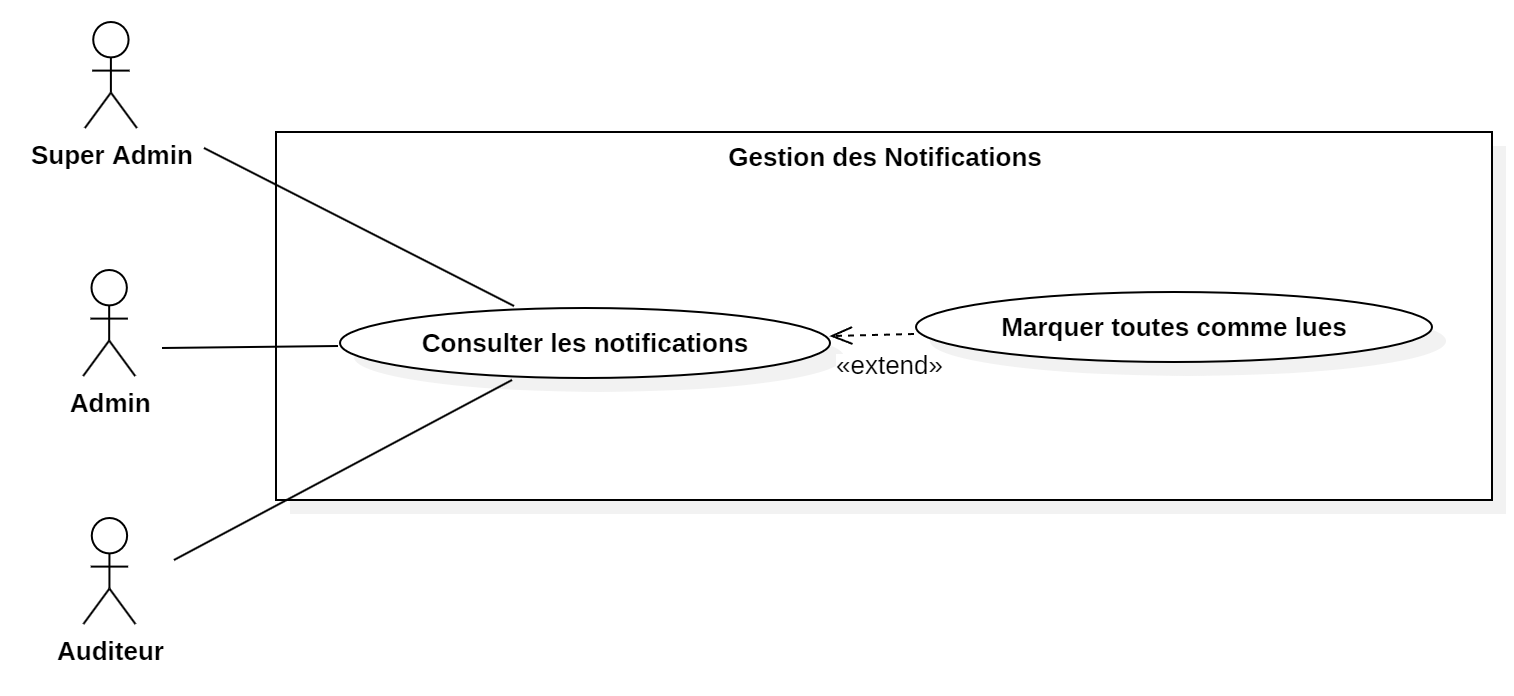
\includegraphics[width=12cm,height=8cm]{images/notificationsuc.png}
    \caption{Diagramme de cas d'utilisation - Gestion des notifications}
\end{figure}

\begin{longtable}{|>{\raggedright\arraybackslash}p{4cm}|>{\raggedright\arraybackslash}p{9cm}|}
\caption{Description textuelle du cas d'utilisation - Gestion des notifications}
\label{tab:manage_notifications_usecase} \\
\hline
\textbf{Cas d'utilisation} & \textbf{Gérer les notifications} \\
\hline
\textbf{Acteur} & Super Admin, Admin, Auditeur \\
\hline
\textbf{Précondition} & Être authentifié \\
\hline
\textbf{Postcondition} & Notifications consultées et marquées comme lues \\
\hline
\textbf{Scénario nominal} & 
1. L'utilisateur clique sur l'icône de notifications \\
& 2. Le système affiche la liste des notifications non lues et lues \\
& 3. L'utilisateur consulte les notifications \\
& 4. L'utilisateur peut marquer toutes les notifications comme lues \\
& 5. Le système met à jour le statut des notifications \\
& 6. Le système met à jour le compteur de notifications non lues \\
\hline
\textbf{Scénario alternatif} & 
- Clic sur notification : navigation vers l'action associée si disponible \\
& - Aucune notification : affichage d'un message approprié \\
& - Mise à jour automatique : rechargement périodique du compteur \\
\hline
\end{longtable}

\subsubsection{Diagramme de cas d'utilisation détaillé de la consultation de l'historique}
\noindent La figure 4.24 présente le diagramme de cas d'utilisation détaillé pour la consultation de l'historique.

\begin{figure}[H]
    \centering
    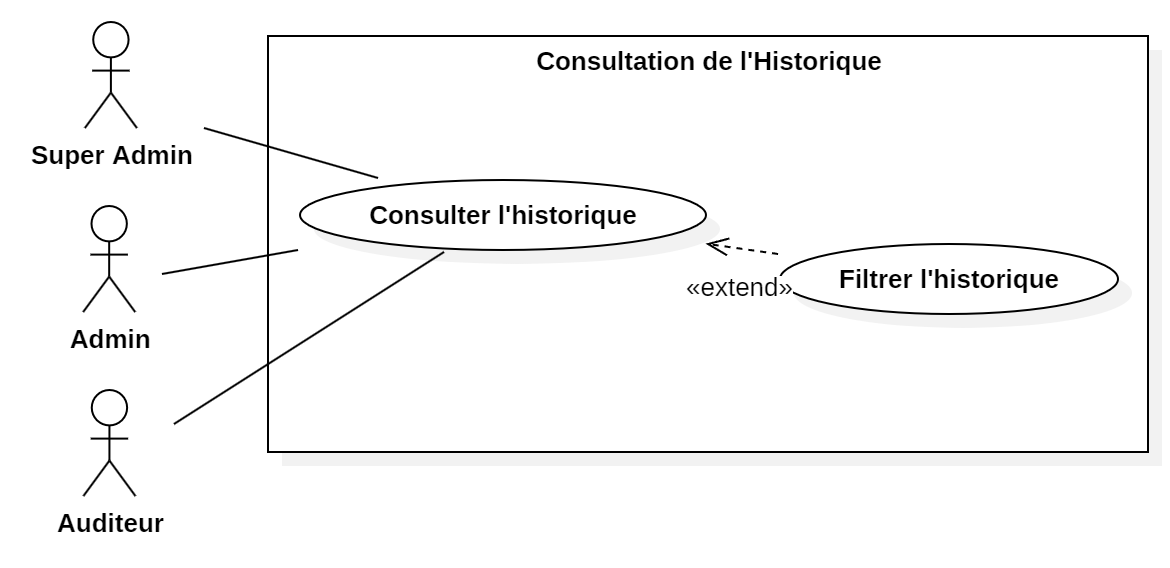
\includegraphics[width=12cm,height=8cm]{images/historyuc.png}
    \caption{Diagramme de cas d'utilisation - Consultation de l'historique}
\end{figure}

\begin{longtable}{|>{\raggedright\arraybackslash}p{4cm}|>{\raggedright\arraybackslash}p{9cm}|}
\caption{Description textuelle du cas d'utilisation - Consultation de l'historique}
\label{tab:consult_history_usecase} \\
\hline
\textbf{Cas d'utilisation} & \textbf{Consulter l'historique} \\
\hline
\textbf{Acteur} & Super Admin, Admin, Auditeur \\
\hline
\textbf{Précondition} & Être authentifié \\
\hline
\textbf{Postcondition} & Historique consulté selon les droits d'accès \\
\hline
\textbf{Scénario nominal} & 
1. L'utilisateur accède à la page d'historique \\
& 2. Le système affiche l'historique selon les droits de l'utilisateur \\
& 3. L'utilisateur peut filtrer par recherche, source, utilisateur ou date \\
& 4. Le système affiche les résultats filtrés avec pagination \\
\hline
\textbf{Scénario alternatif} & 
- Super Admin : accès à tout l'historique du système \\
& - Admin : accès à l'historique de son entreprise \\
& - Auditeur : accès uniquement à son propre historique \\
& - Filtres : application combinée de plusieurs critères \\
\hline
\end{longtable}

\subsubsection{Diagramme de cas d'utilisation détaillé de la consultation des statistiques}
\noindent La figure 4.25 présente le diagramme de cas d'utilisation détaillé pour la consultation des statistiques.

\begin{figure}[H] 
    \centering
    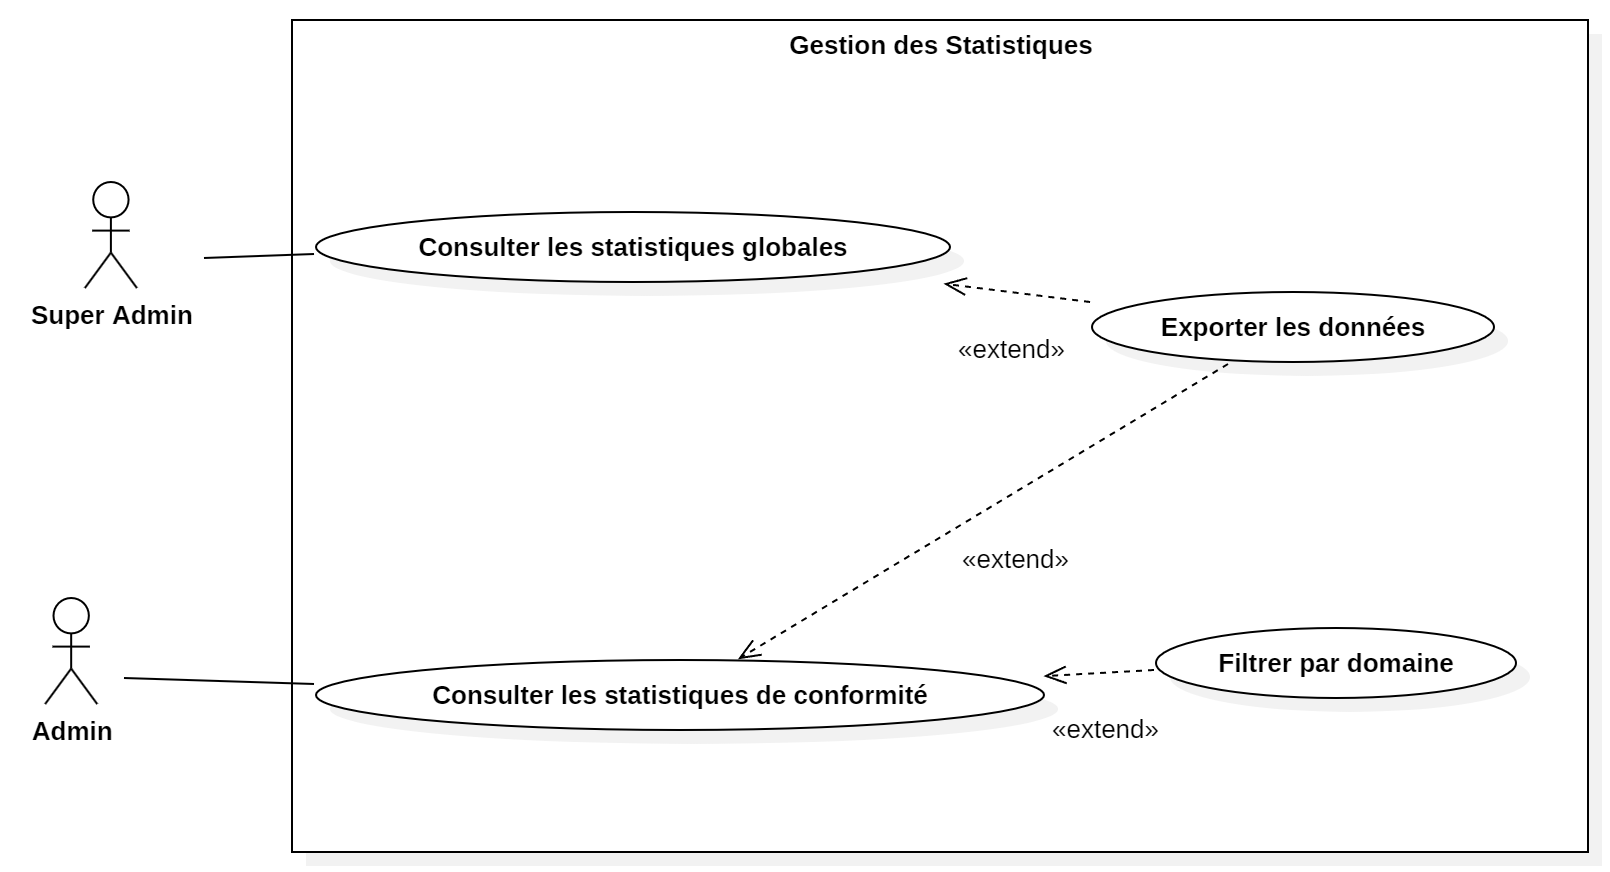
\includegraphics[width=12cm,height=8cm]{images/statisticsuc.png}
    \caption{Diagramme de cas d'utilisation - Consultation des statistiques}
\end{figure}

\begin{longtable}{|>{\raggedright\arraybackslash}p{4cm}|>{\raggedright\arraybackslash}p{9cm}|}
\caption{Description textuelle du cas d'utilisation - Consultation des statistiques}
\label{tab:consult_statistics_usecase} \\
\hline
\textbf{Cas d'utilisation} & \textbf{Consulter les statistiques} \\  % untouched
\hline
\textbf{Acteur} & Super Admin, Admin \\
\hline
\textbf{Précondition} & Être correctement authentifié en tant que Super Admin ou Admin \\ % subtle addition
\hline
\textbf{Postcondition} & Statistiques consultées selon les droits d'accès disponibles \\ % subtle addition
\hline
\textbf{Scénario nominal} & 
1. L'utilisateur accède à la page de statistiques \\
& 2. Le système affiche les statistiques selon les droits de l'utilisateur \\
& 3. L'utilisateur consulte les graphiques et indicateurs \\
& 4. L'utilisateur peut filtrer les données si applicable \\
& 5. Le système affiche les résultats actualisés \\
\hline
\textbf{Scénario alternatif} & 
- Super Admin : accès aux statistiques globales du système (entreprises, utilisateurs, demandes) \\
& - Admin : accès aux statistiques de conformité de son entreprise (textes, exigences, actions) \\
& - Filtrage par domaine : pour les Admins, filtrage des statistiques par domaine spécifique \\
& - Aucune donnée : affichage d'un message approprié \\
\hline
\end{longtable}

\subsection{Conception}
\noindent Dans cette partie, nous passons à la seconde phase de notre sprint, qui consiste à aborder la conception détaillée du système. Notre objectif principal est de créer les diagrammes de séquence correspondant à cette étape, afin de représenter clairement le déroulement des interactions entre les différents acteurs et le système.


\subsubsection{Diagramme de séquence pour le scénario de création d'une revue de direction}
\begin{figure}[H]
    \centering
    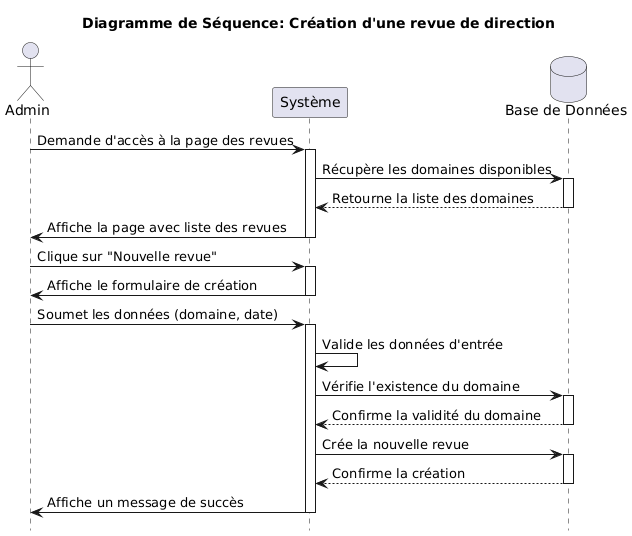
\includegraphics[width=10cm,height=9cm]{images/createrevueseq.png}
    \caption{Diagramme de séquence pour le scénario de création d'une revue de direction}
\end{figure}

\subsubsection{Diagramme de séquence pour le scénario de consultation des revues de direction}
\begin{figure}[H]
    \centering
    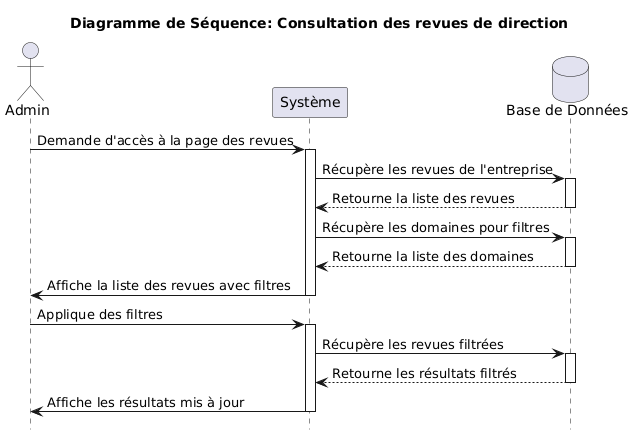
\includegraphics[width=10cm,height=9cm]{images/consultrevueseq.png}
    \caption{Diagramme de séquence pour le scénario de consultation des revues de direction}
\end{figure}

\subsubsection{Diagramme de séquence pour le scénario de modification d'une revue de direction}
\begin{figure}[H]
    \centering
    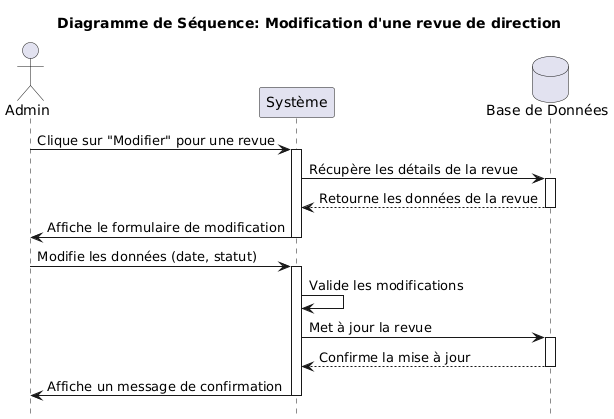
\includegraphics[width=10cm,height=9cm]{images/modifyrevueseq.png}
    \caption{Diagramme de séquence pour le scénario de modification d'une revue de direction}
\end{figure}

\subsubsection{Diagramme de séquence pour le scénario de suppression d'une revue de direction}
\begin{figure}[H]
    \centering
    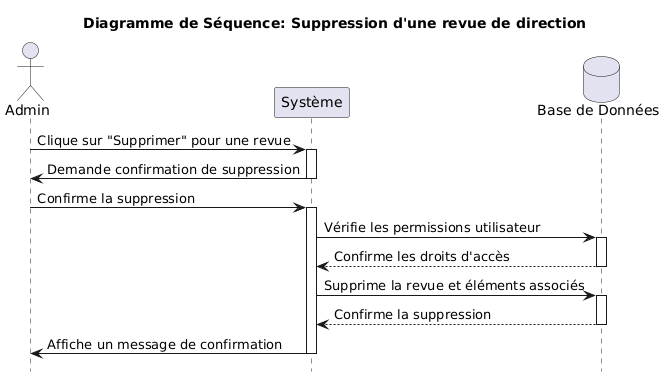
\includegraphics[width=10cm,height=9cm]{images/deleterevueseq.png}
    \caption{Diagramme de séquence pour le scénario de suppression d'une revue de direction}
\end{figure}

\subsubsection{Diagramme de séquence pour le scénario de changement de statut d'une revue}
\begin{figure}[H]
    \centering
    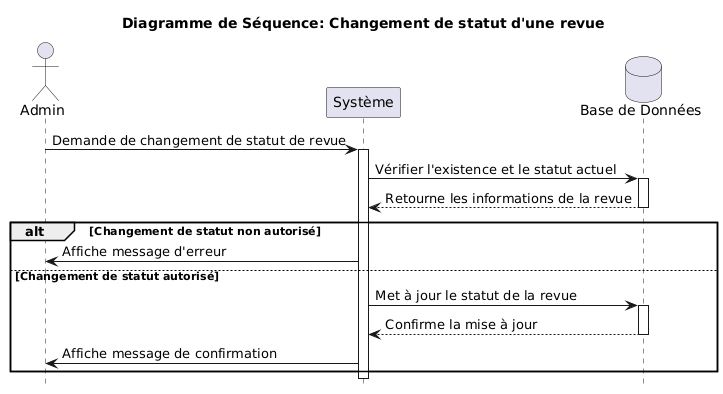
\includegraphics[width=9cm,height=9cm]{images/changestatusrevueseq.png}
    \caption{Diagramme de séquence pour le scénario de changement de statut d'une revue}
\end{figure}

\subsubsection{Diagramme de séquence pour le scénario de consultation des éléments d'une revue}
\begin{figure}[H]
    \centering
    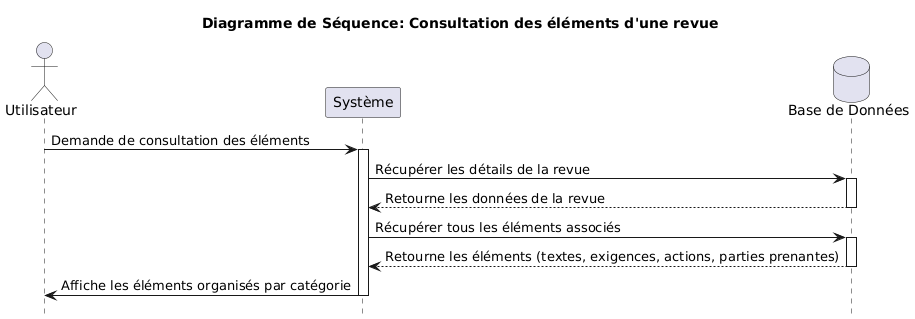
\includegraphics[width=10cm,height=7cm]{images/consultelementrevueseq.png}
    \caption{Diagramme de séquence pour le scénario de consultation des éléments d'une revue}
\end{figure}

\subsubsection{Diagramme de séquence pour le scénario d'ajout d'un élément à une revue}
\begin{figure}[H]
    \centering
    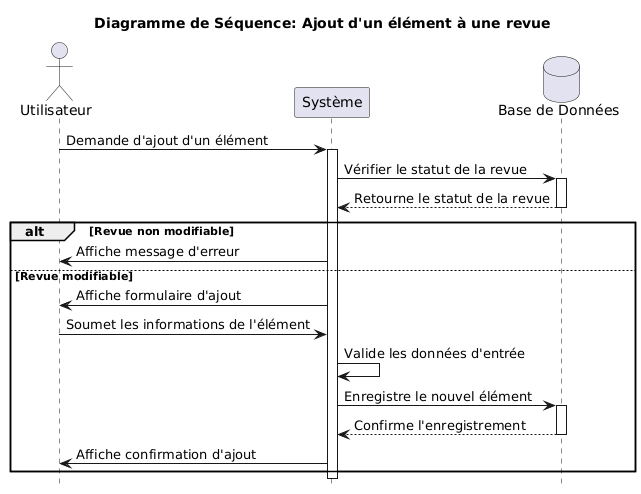
\includegraphics[width=10cm,height=9cm]{images/addelementrevueseq.png}
    \caption{Diagramme de séquence pour le scénario d'ajout d'un élément à une revue}
\end{figure}

\subsubsection{Diagramme de séquence pour le scénario de modification d'un élément de revue}
\begin{figure}[H]
    \centering
    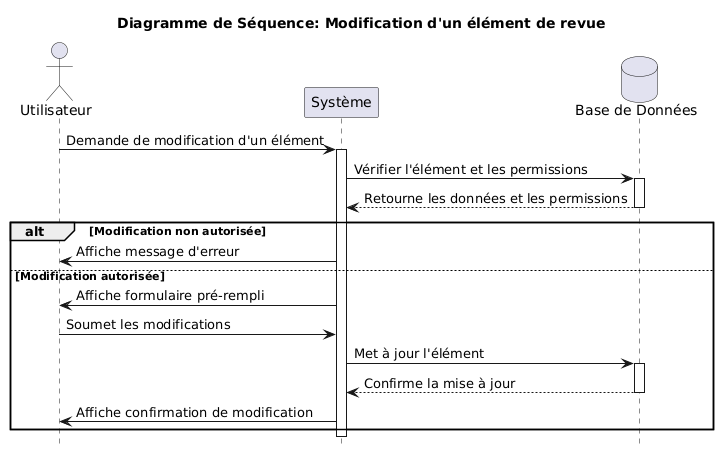
\includegraphics[width=10cm,height=9cm]{images/modifyelementrevueseq.png}
    \caption{Diagramme de séquence pour le scénario de modification d'un élément de revue}
\end{figure}

\subsubsection{Diagramme de séquence pour le scénario de suppression d'un élément de revue}
\begin{figure}[H]
    \centering
    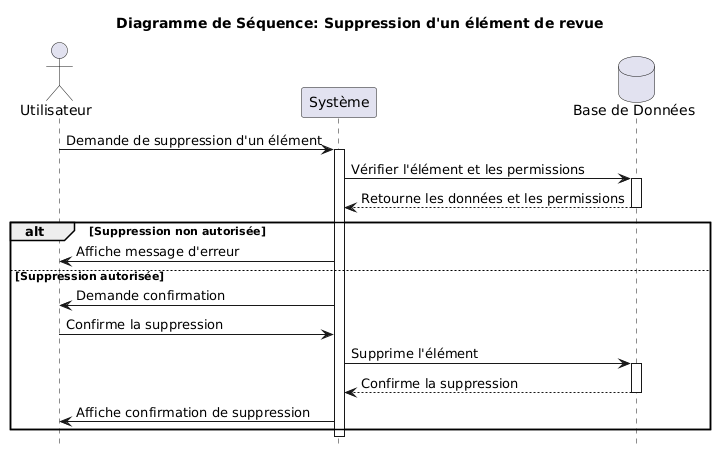
\includegraphics[width=10cm,height=9cm]{images/deleteelementrevueseq.png}
    \caption{Diagramme de séquence pour le scénario de suppression d'un élément de revue}
\end{figure}

\subsubsection{Diagramme de séquence pour le scénario de génération de PDF d'une revue}
\begin{figure}[H]
    \centering
    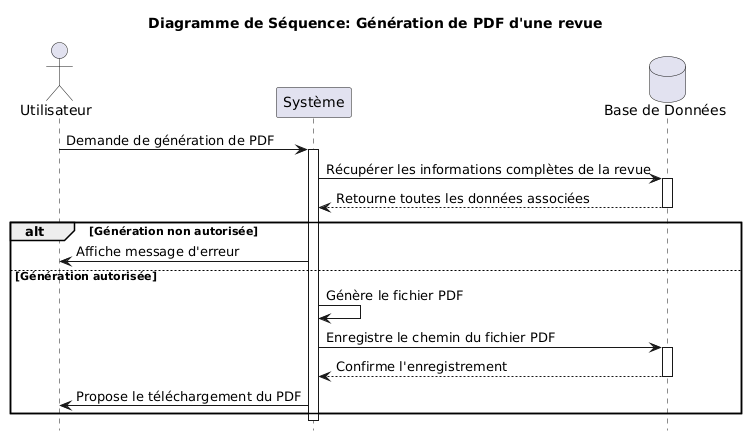
\includegraphics[width=10cm,height=9cm]{images/generatepdfrevueseq.png}
    \caption{Diagramme de séquence pour le scénario de génération de PDF d'une revue}
\end{figure}


\subsubsection{Diagramme de séquence pour le scénario de consultation des notifications}
\begin{figure}[H]
    \centering
    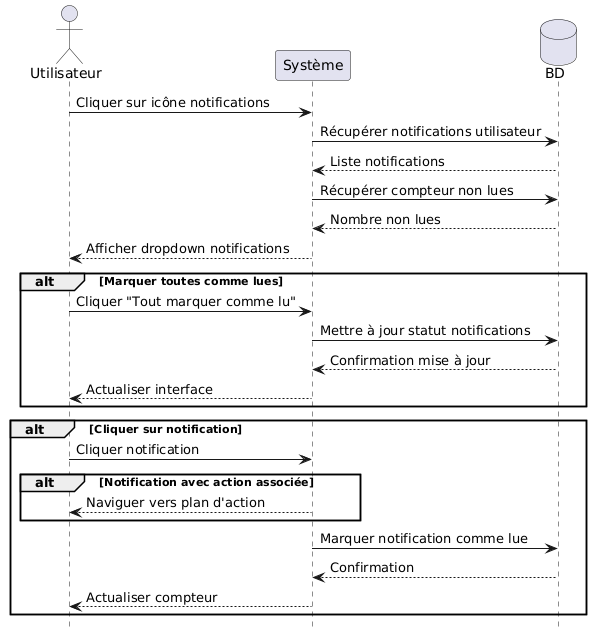
\includegraphics[width=10cm,height=9cm]{images/consultnotificationsseq.png}
    \caption{Diagramme de séquence pour le scénario de consultation des notifications}
\end{figure}

\subsubsection{Diagramme de séquence pour le scénario de marquage de toutes les notifications comme lues}
\begin{figure}[H]
    \centering
    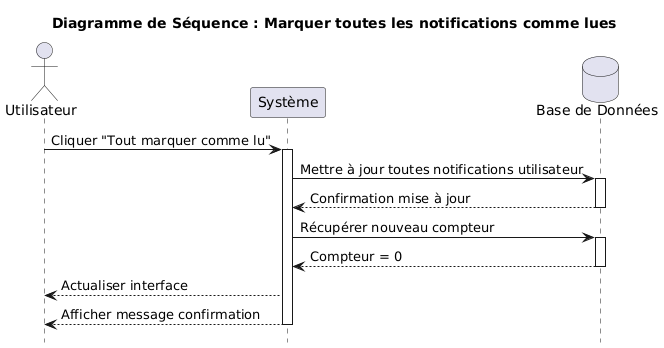
\includegraphics[width=10cm,height=8cm]{images/markallreadseq.png}
    \caption{Diagramme de séquence pour le scénario de marquage de toutes les notifications comme lues}
\end{figure}

\subsubsection{Diagramme de séquence pour le scénario de consultation de l'historique}
\begin{figure}[H]
    \centering
    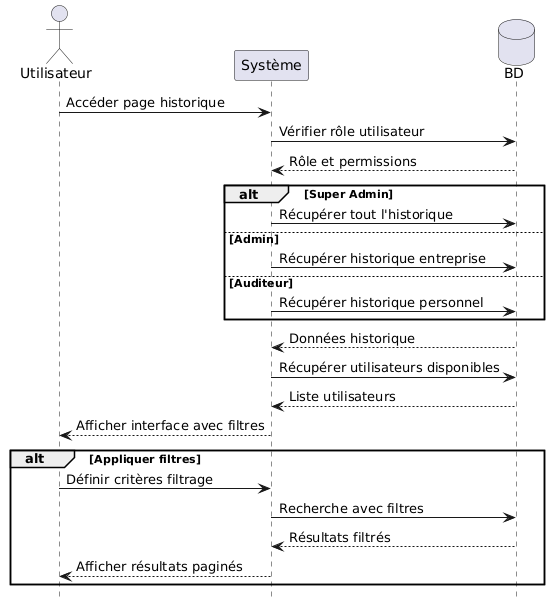
\includegraphics[width=10cm,height=9cm]{images/consulthistoryseq.png}
    \caption{Diagramme de séquence pour le scénario de consultation de l'historique}
\end{figure}


\subsubsection{Diagramme de séquence pour le scénario de consultation des statistiques globales}
\begin{figure}[H]
    \centering
    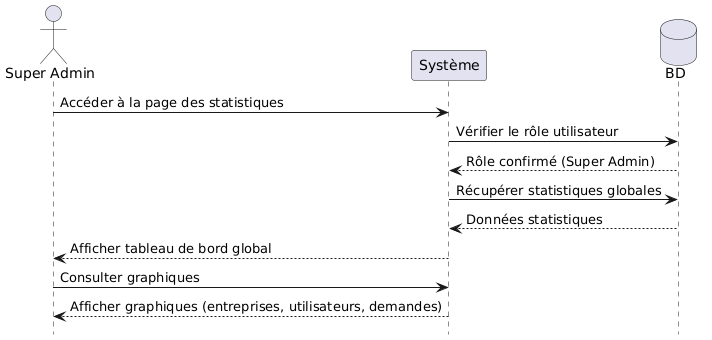
\includegraphics[width=9cm,height=8cm]{images/consultglobalstatsseq.png}
    \caption{Diagramme de séquence pour le scénario de consultation des statistiques globales}
\end{figure}

\subsubsection{Diagramme de séquence pour le scénario de consultation des statistiques de conformité)}
\begin{figure}[H]
    \centering
    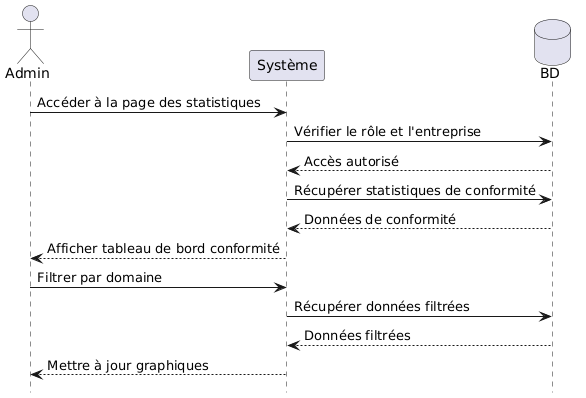
\includegraphics[width=10cm,height=9cm]{images/consultcompliancestatsseq.png}
    \caption{Diagramme de séquence pour le scénario de consultation des statistiques de conformité}
\end{figure}

\subsection{Réalisation}
\noindent Dans cette section, nous vous présenterons les résultats de ce sprint sous forme d'une série de captures d'écran illustrant différentes interfaces que nous avons développées.

\subsubsection{Interface de gestion des revues de direction}
\noindent La figure 4.39 présente l'interface de gestion des revues de direction permettant de consulter, créer et gérer les revues.

\begin{figure}[H]
    \centering
    \includegraphics[width=14cm,height=9cm]{images/revuedirectioninterface.PNG}
    \caption{Interface de gestion des revues de direction}
\end{figure}

\subsubsection{Interface de création d'une revue de direction}
\noindent La figure 4.40 présente l'interface de création d'une nouvelle revue de direction avec sélection du domaine et de la date.

\begin{figure}[H]
    \centering
    \includegraphics[width=14cm,height=9cm]{images/createrevuemodal.PNG}
    \caption{Interface de création d'une revue de direction}
\end{figure}

\subsubsection{Interface de détails d'une revue}
\noindent La figure 4.43 présente l'interface de consultation des détails d'une revue de direction avec tous les éléments associés.

\begin{figure}[H]
    \centering
    \includegraphics[width=13cm,height=8cm]{images/revuedetails.PNG}
    \caption{Interface de détails d'une revue}
\end{figure}

\subsubsection{Interface d'ajout d'un élément à une revue}
\noindent La figure 4.44 présente l'interface d'ajout d'un élément (texte légal, exigence, action ou partie prenante) à une revue.

\begin{figure}[H]
    \centering
    \includegraphics[width=12cm,height=7cm]{images/addelementmodal.PNG}
    \caption{Interface d'ajout d'un élément à une revue}
\end{figure}

\subsubsection{Interface du dropdown des notifications}
\noindent La figure 4.47 présente l'interface du dropdown des notifications permettant de consulter et gérer les notifications.

\begin{figure}[H]
    \centering
    \includegraphics[width=10cm,height=6cm]{images/notificationsdropdown.PNG}
    \caption{Interface du dropdown des notifications}
\end{figure}

\subsubsection{Interface de consultation de l'historique}
\noindent La figure 4.49 présente l'interface de consultation de l'historique avec filtres et pagination.

\begin{figure}[H]
    \centering
    \includegraphics[width=14cm,height=9cm]{images/historyinterface.PNG}
    \caption{Interface de consultation de l'historique}
\end{figure}

\subsubsection{Interface des statistiques globales (Super Admin)}
\noindent La figure 4.53 présente l'interface des statistiques globales du système accessible au Super Admin.

\begin{figure}[H]
    \centering
    \includegraphics[width=12cm,height=7cm]{images/globalstatsinterface.PNG}
    \caption{Interface des statistiques globales}
\end{figure}

\subsubsection{Interface des statistiques de conformité (Admin)}
\noindent La figure 4.54 présente l'interface des statistiques de conformité de l'entreprise accessible à l'Admin.

\begin{figure}[H]
    \centering
    \includegraphics[width=12cm,height=7cm]{images/compliancestatsinterface.PNG}
    \caption{Interface des statistiques de conformité}
\end{figure}

\section*{CONCLUSION}
\noindent Cette deuxième release a permis de compléter le système « Prévention Plus » avec l'implémentation des fonctionnalités de gestion des abonnements, des textes réglementaires, de l'évaluation de conformité, des plans d'action, des revues de direction, des notifications, de l'historique et des statistiques. Ces fonctionnalités renforcent la capacité des utilisateurs à gérer efficacement les processus de conformité et d'évaluation, tout en assurant une traçabilité et une analyse approfondie des données.